
\chapter{Inference for categorical data}
\label{inferenceForCategoricalData}

Statistical inference is concerned primarily with understanding the
accuracy of parameter estimates. While the equations and details change
depending on the setting, the foundations for inference are the same
throughout all of statistics. We introduce these common themes in
Sections~\ref{pointEstimates}-\ref{hypothesisTesting} by discussing
inference about the population proportion, $p$.
In Sections~\ref{}-\ref{}, we'll expand
to the application of comparing two proportions against each other.
Finally, we'll complete this chapter by analyzing categorical data
where there are many levels.

Each of the ideas in this chapter are applicable to a broad set of
applications and new contexts. We'll expand on these ideas in later
chapters.

\Comment{Do additional checks to confirm that the term
\emph{standard error} is being used consistently rather than
\emph{standard deviation}.}




%__________________
\section[Point estimates and sampling variability]
    {Point estimates and sampling \\ variability}
    %\sectionvideohref{youtube-DNIauUrRIEM&list=PLkIselvEzpM7Pjo94m1e7J5jkIZkbQAl4}~\sectionslideshref{gdoc_os3_slides_4-1}}
\label{pointEstimates}

\index{data!solar survey|(}

\newcommand{\pewsolarpollsize}{1000}
\newcommand{\pewsolarpollprop}{0.887}
\newcommand{\pewsolarpollpropcomplement}{0.113}
\newcommand{\pewsolarpollpercent}{88.7}
\newcommand{\pewsolarpollpercentcomplement}{11.3}
\newcommand{\pewsolarpollcount}{887}
\newcommand{\pewsolarpollcountcomplement}{113}
\newcommand{\pewsolarpollse}{0.0100}

Pew Research conducted a poll in 2018 gauging public opinion of
American adults on solar and wind energy. They surveyed 1,000
Americans and found that \pewsolarpollpercent{}\% of respondents
favored expanding
solar energy.\footnote{The full survey's sample size was 2541,
and we've taken a subsample. To find the survey details, see\\
\oiRedirect{textbook-pew_2018_poll_on_solar_and_wind_expansion}{http://www.pewinternet.org/2018/05/14/majorities-see-government-efforts-to-protect-the-environment-as-insufficient}}
\Comment{The redirect link in the footnote needs to be confirmed as
working.}
One of the most common questions people ask about polls is
\begin{quote}
If the poll was based on only a couple thousand people, how reliable is it?
\end{quote}
If we took another poll, we wouldn't get the exact same answer.
Ultimately, it's unlikely that the actual proportion of Americans
who support expanding solar energy is \emph{exactly}
\pewsolarpollpercent{}\%, but it's probably something close to
\pewsolarpollpercent{}\%.

In this section, we discuss what a point estimate like
\pewsolarpollpercent{}\% represents
and the uncertainty associated with such an estimate. We'll also
be using some new notation and terminology:
\begin{itemize}
\item The population proportion will be written as $p$, which
    is called a \term{parameter} of the population. In the solar
    survey, $p$ represents the proportion of \emph{all}
    American adults who support solar energy. It's rare
    that we know the parameter. Instead, we often
    take a sample and compute an estimate.
\item Using Pew Research sample, we can estimate that the proportion
    of American adults who support expanding solar energy is
    \pewsolarpollpercent{}\%.
    This is called the \term{sample proportion}, and it gets a special
    label of $\hat{p}$ (spoken as \emph{p-hat}).
\item The \termsub{size of a sample}{sample size} will generally
    be denoted by $n$. In the case of this Pew Research poll,
    $n = \pewsolarpollsize{}$.
\end{itemize}

\subsection{Point Estimates}

\index{point estimate|(}

The sample proportion $\hat{p} = \pewsolarpollprop{}$ is called
the \term{point estimate} of the parameter $p$, since based
on the sample, this is our single best estimate of $p$.

The poll provides a \term{point estimate} of the actual proportion
of American adults that support expanding solar energy.
This estimate of \pewsolarpollpercent{}\% is unlikely to be perfect,
and it's quite possible for the \term{true proportion}
(a.k.a. the population proportion) to be a little lower
or a little higher. The difference between a point estimate
and the parameter is called the estimate's \term{error}.

\Comment{Should we aggressively cut out the usage of ``true''
  in the way it is used above?}

The error varies from one sample to the next: maybe
in one sample it is 1\% too low while in another
it is 3\% too high. Unfortunately, we rarely know the direction
or size of the error in our estimates, so instead we focus
on understanding what kinds of errors are typical.


\subsection{Understanding the variability of a point estimate}
\label{simulationForUnderstandingVariabilitySection}

We want to understand \emph{how does the
sample proportion $\hat{p}$ behave when the population
proportion is about \pewsolarpollprop{}}. We could
run the survey again to see how consistent the results
are, but who has the time and money for that? Instead,
we can investigate the properties of $\hat{p}$ using simulations.

To simulate the sample, we'll suppose that the population
proportion is exactly \pewsolarpollpercent{}\%.
%Now, we know
%the population proportion isn't exactly \pewsolarpollpercent\%,
%but we do expect it to be close, so this simulation will offer
%us some insights about the property of $\hat{p}$.
%If we took a random sample
%from this population, how accurate would the point estimate be?
Here's how we might simulate it:
\begin{enumerate}
\item There were about 250 million American adults in 2018.
    On 250 million pieces of paper, write ``support''
    on \pewsolarpollpercent{}\% of them and ``not'' on
    the other \pewsolarpollpercentcomplement{}\%.
\item Mix up the pieces of paper and pull out \pewsolarpollsize{}
    pieces to represent our sample of 1000 American adults.
\item Compute the fraction of the sample that say ``support''.
\end{enumerate}
Any volunteers to conduct this simulation? Probably not. Running
this simulation with 250 million pieces of paper would be
time-consuming and very costly, but we can simulate it
using computer code; we've written a short program in the
footnote.\footnote{Code using the statistical software called \R: \\
\texttt{\# 1. Create a set of 250 million entries,
where 89\% of them are "support" and 11\% are "not". \\
possible\_entries <- rep(c("support", "not"),
    c(\pewsolarpollprop{}, \pewsolarpollpropcomplement{}) * 250e6)\\
\# 2. Sample \pewsolarpollsize{} of the entries. \\
sampled\_entries <- sample(possible\_entries, \pewsolarpollsize{}) \\
\# 3. Count the number that are "justified", then divide
by the sample size. \\
sum(sampled\_entries == "justified") / \pewsolarpollsize{}}}
In this simulation, the sample gave a point estimate of
$\hat{p}_1 = 0.901$. We~know the population proportion
in this simulation is $p = \pewsolarpollprop{}$, so we know
the estimate had an error of +0.014.

One simulation isn't enough to get a sense of the null
distribution, so we should run more simulations. In a second
simulation, we get $\hat{p}_2 = 0.892$, which has an error of
+0.005.
In another, $\hat{p}_3 = 0.885$ for an error of -0.002. And in another,
an estimate of $\hat{p}_4 = 0.866$ with an error of -0.021.
With the help of a computer, we've run the simulation 10,000 times
and created a histogram of the results from all 10,000 simulations
in Figure~\ref{sampling_10k_prop_887p}. This
distribution of sample proportions is called a
\term{sampling distribution}.
%\footnote{Here is the code for 10,000 simulations: \\
%\texttt{people <- rep(c("justified", "not"), c(0.56, 0.44) * 247e6) \\
%sim.results <- c() \\
%for (i in 1:10000) \{ \\
%\ \hspace{5mm}sampled.people <- sample(people, 1000) \\
%\ \hspace{5mm}sim.results[i] <- mean(sampled.people == "justified") \\
%\} \\
%hist(sim.results, 20)} \\
%(There's actually a more efficient way to write this code, but we have provided you the long version!)}
We can characterize this sampling distribution as follows:
\begin{description}
\item[Center.] The center of the distribution is
    $\bar{x}_{\hat{p}} = \pewsolarpollprop{}0$, which is the same as the
    population proportion.
    That~is, we see that the sample proportion is an
    \term{unbiased estimate} of the population proportion.
\item[Spread.] The standard deviation of the distribution
    is $s_{\hat{p}} = \pewsolarpollse{}$. When we're talking about
    a sampling distribution or the variability of
    a point estimate, we typically use the term
    \termsub{standard error}{standard error (SE)}
    rather than \emph{standard deviation},
    and the notation $SE_{\hat{p}}$ is used for the standard
    error associated with the sample proportion.
\item[Shape.] The distribution is symmetric and bell-shaped,
    and it \emph{resembles a normal distribution}.
\end{description}
These findings are very encouraging! When the population
proportion is $p = \pewsolarpollprop{}$ and the sample size is
$n = \pewsolarpollsize{}$,
the sample proportion $\hat{p}$ tends to give a pretty good estimate
of the population proportion. We also have this interesting observation
that the histogram resembles a normal distribution.

\begin{figure}
   \centering
   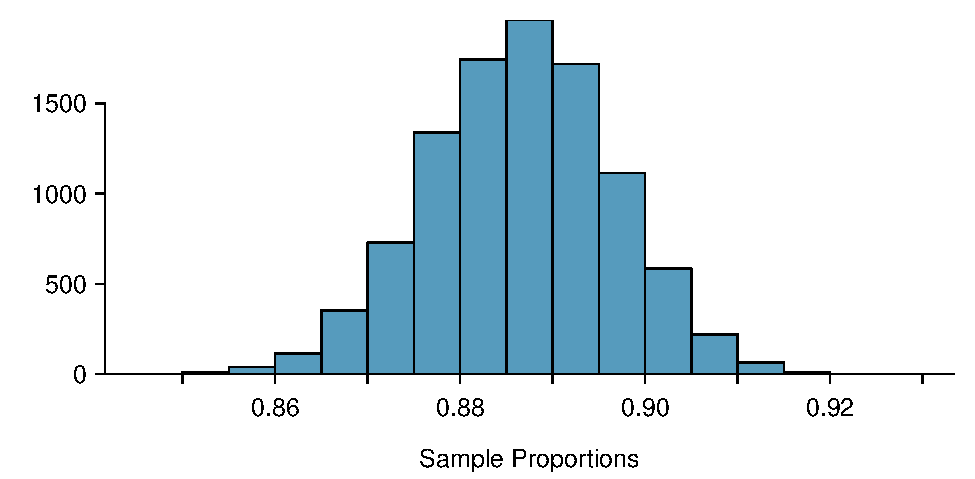
\includegraphics[width=0.8\textwidth]{ch_inference_for_props/figures/sampling_10k_prop_887p/sampling_10k_prop_887p}
   \caption{A histogram of 10,000 sample proportions, where each
       sample is taken from a population where the population of
       proportion is \pewsolarpollprop{} and the sample size is
       $n = \pewsolarpollsize{}$.}
   \label{sampling_10k_prop_887p}
\end{figure}

\begin{tipBox}{\tBoxTitle{Sampling distributions are something we
    keep in mind, even if they are never observed}
  In real-world applications, we never actually observe the
  sampling distribution, yet it is useful to always think of
  the sample proportion as coming from such a distribution.
  Understanding the distribution will help us characterize
  and make sense of the individual point estimate that we
  do observe.}
\end{tipBox}

\begin{example}{If we used a much smaller sample size of $n = 50$,
would you guess that the standard error for $\hat{p}$ would be larger
or smaller than when we used $n = \pewsolarpollsize{}$?}
\label{smallerSampleWhatHappensToPropErrorExercise}
Intuitively, it seems like more data is better
than less data, and generally that is correct! The typical error
when $p = \pewsolarpollprop{}$ and $n = 50$ would be larger
than the error we would expect when $n = \pewsolarpollsize{}$.
\end{example}

%\noindent
Example~\ref{smallerSampleWhatHappensToPropErrorExercise}
highlights an important property: a bigger sample
tends to provide a more precise point estimates than a smaller sample.

\index{point estimate|)}


\subsection{Central Limit Theorem}

The distribution in
Figure~\ref{sampling_10k_prop_887p} looks an awful lot like
a normal distribution. That is no anomaly; it is the result
of a general principle called the \term{Central Limit Theorem}.
\index{Central Limit Theorem!proportion|textbf}

\begin{termBox}{\tBoxTitle{Central Limit Theorem for proportions
    \& the success-failure condition}
When observations are independent and the sample size is
sufficiently large, the sample proportion $\hat{p}$ will tend
to follow a normal distribution with the following mean and
standard error:
\begin{align*}
  \mu_{\hat{p}} &= p
  &SE_{\hat{p}} &= \sqrt{\frac{p (1 - p)}{n}}
\end{align*}
The sample size is typically considered sufficiently large when
$np \geq 10$ and $n(1-p) \geq 10$, which is called the
\term{success-failure condition}.} %since $np$ represents the
%number of expected \emph{successes} and $n(1-p)$ the expected
%number of \emph{failures}.}
\end{termBox}

The Central Limit Theorem is incredibly important, and it provides
a foundation for the rest of this book. As we begin applying
this principle, be mindful of the two requirements:
the observations must be independent, and the the sample size must
be sufficiently large such that $np \geq 10$ and $n(1-p) \geq 10$.

\begin{example}{Earlier we estimated the mean and standard
error of the $\hat{p}$'s using simulated data when
$p = \pewsolarpollprop{}$ and $n = \pewsolarpollsize{}$.
Confirm that the distribution is approximately
normal.}\label{sample_p887_n1000_confirm_normal}
\begin{description}
\item[Independence.] There are $n = \pewsolarpollsize{}$
    observations for each
    sample proportion $\hat{p}$, and each of those observations
    are independent draws. \emph{The most common way for
    observations to be considered independent is if they are from
    a simple random sample.}
    \index{independent}
    \index{independence}
    \index{Central Limit Theorem|independence}
\item[Success-failure condition.] We can confirm the sample size
    is sufficiently large by checking the success-failure condition
    and confirming each of the following values are greater than 10:
    \begin{align*}
    np &= \pewsolarpollsize{} \times \pewsolarpollprop{}
        = \pewsolarpollcount{}
    &n(1-p) &= \pewsolarpollsize{} \times (1 - \pewsolarpollprop{})
        = \pewsolarpollcountcomplement{}
    \end{align*}
\end{description}
Both of the independence and success-failure conditions are
satisfied, so the Central Limit Theorem applies and the normal
distribution is reasonable in this context!
\end{example}

\begin{example}{Compute the theoretical mean and standard error
of the $\hat{p}$'s when
$p = \pewsolarpollprop{}$ and $n = \pewsolarpollsize{}$,
according to the
Central Limit Theorem.}\label{sample_p887_n1000_mean_se}
The mean of the $\hat{p}$'s is simply the population proportion:
$\mu_{\hat{p}} = \pewsolarpollprop{}$.

The calculation of the standard error of $\hat{p}$ uses
the following formula:
\begin{align*}
SE_{\hat{p}}
    = \sqrt{\frac{p (1 - p)}{n}}
    = \sqrt{\frac{\pewsolarpollprop{} (1 - \pewsolarpollprop{})}{1000}}
    = \pewsolarpollse{}
\end{align*}
\end{example}

\begin{example}{Estimate how frequently the sample proportion
$\hat{p}$ should be within 0.02 (2\%) of the population value,
$p = \pewsolarpollprop{}$. Based on
Examples~\ref{sample_p887_n1000_confirm_normal}
and~\ref{sample_p887_n1000_mean_se}, we know that the distribution is
$N(\mu_{\hat{p}} = \pewsolarpollprop{}, SE_{\hat{p}} = \pewsolarpollse{})$.}
\label{sampling_10k_prop_887p-prop_from_867_to_907}
After so much practice in Section~\ref{normalDist},
this example will hopefully feel familiar!
We would like to understand the fraction of $\hat{p}$'s
between 0.867 and 0.907:
\begin{center}
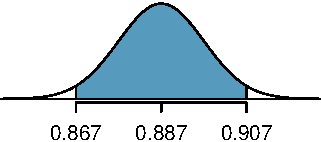
\includegraphics[width=60mm]{ch_inference_for_props/figures/p-hat_from_867_and_907/p-hat_from_867_and_907}
\end{center}
With $\mu_{\hat{p}} = \pewsolarpollprop{}$ and
$SE_{\hat{p}} = \pewsolarpollse{}$,
we can compute the Z-score for both the left and right cutoffs:
\begin{align*}
Z_{0.867} &= \frac{0.867 - \pewsolarpollprop{}}{\pewsolarpollse{}} = -2
&Z_{0.907} &= \frac{0.907 - \pewsolarpollprop{}}{\pewsolarpollse{}} = 2
\end{align*}
We can use either statistical software, a graphing calculator,
or a table to find the areas to the tails, and in any case we
will find that they are each 0.0228. The total tail areas are
$2 \times 0.0228 = 0.0456$, which leaves the shaded area of
0.9544. That is, about 95.44\% of the sampling distribution
in Figure~\ref{sampling_10k_prop_887p} is within $\pm0.02$
of the simulation population proportion, $p = \pewsolarpollprop{}$.
%of these
%cutoffs and compute the difference of these areas
%to get the central area:
%\begin{center}
%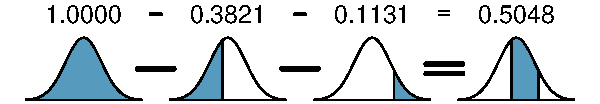
\includegraphics[width=60mm]{ch_inference_for_props/figures/p-hat_from_53_and_59_computation/p-hat_from_53_and_59_computation}
%\end{center}
\end{example}

\begin{exercise}
In Example~\ref{smallerSampleWhatHappensToPropErrorExercise}
we discussed how a smaller sample would tend
to produce a less reliable estimate. Explain how this intuition
is reflected in the formula for
$SE_{\hat{p}} = \sqrt{\frac{p (1 - p)}{n}}$.\footnote{Since the
sample size $n$ is in the denominator of the fraction (on the
bottom of the fraction), a bigger sample size means the entire
expression when calculated will tend to be smaller. That is,
a larger sample size would correspond to a smaller standard error.}
\end{exercise}

%In Example~\ref{sampling_10k_prop_56p}, we applied a general
%principle called the \term{Central Limit Theorem}
%\hiddenterm{Central Limit Theorem!proportions} when
%we used the normal distribution as an approximation.


\subsection{Applying the Central Limit Theorem to a real-world setting}

Think back to the 2018 poll where
$\hat{p} = \pewsolarpollprop{}$ of American adults favored
expanding solar energy. We might wonder: does the sample
proportion from the poll approximately follow a normal
distribution?
We check the conditions from the Central Limit Theorem:
\begin{description}
\item[Independence.] The poll is a simple random sample of
    American adults, which means that the observations are
    independent.
\item[Success-failure condition.] To check this condition,
    we need the population proportion, $p$, to check if both
    $np$ and $n(1-p)$ are greater than 10. However, we do not
    know the value of $p$; that's exactly why the pollsters
    took a sample! In cases like these, we often use $\hat{p}$
    as our next best way to check the success-failure condition:
    \begin{align*}
    n\hat{p} &= \pewsolarpollsize{} \times \pewsolarpollprop{}
        = \pewsolarpollcount{}
    &n (1 - \hat{p}) &= \pewsolarpollsize{} \times (1 - \pewsolarpollprop{})
        = \pewsolarpollcountcomplement{}
    \end{align*}
    While we cannot check the condition with $p$,
    $\hat{p}$ acts as a reasonable substitute, and we are comfortably
    above the minimums of 10.
\end{description}

This \term{substitution approximation} of using $\hat{p}$ in
place of $p$ will also be useful when computing the standard error
of the sample proportion in many situations:
\begin{align*}
SE_{\hat{p}}
    = \sqrt{\frac{p (1 - p)}{n}}
    \approx \sqrt{\frac{\hat{p} (1 - \hat{p})}{n}}
    \approx \sqrt{\frac{\pewsolarpollprop{}
        (1 - \pewsolarpollprop{})}{\pewsolarpollsize{}}}
    = \pewsolarpollse{}
\end{align*}
This substitution approximation technique is useful in many
situations.
%\footnote{There are additional methods
%for proportions that perform some correction for the substitution
%approximation. However, we leave those proportion methods for
%a future course.}




%__________________
\section[Confidence interval for a sample proportion]{Confidence
    intervals for\\a sample proportion} % \sectionvideohref{youtube-FUaXoKdCre4&list=PLkIselvEzpM7Pjo94m1e7J5jkIZkbQAl4}~\sectionslideshref{gdoc_os3_slides_4-2}}
\label{confidenceIntervals}

\index{confidence interval|(}

The sample proportion $\hat{p}$ provides a single plausible value
for the population proportion $p$. However, the sample proportion
isn't perfect and will have some \emph{standard error}
associated with it. Instead of supplying just this point estimate
of the population proportion, a next logical step would be
to provide a plausible \emph{range of values}.

\subsection{Capturing the population parameter}

A plausible range of values for the population parameter
is called a \term{confidence interval}.

Using only a point estimate is like fishing in a murky
lake with a spear, and using a confidence interval is
like fishing with a net. We can throw a spear where we
saw a fish, but we will probably miss. On the other hand,
if we toss a net in that area, we have a good chance of
catching the fish.

If we report a point estimate $\hat{p}$, we probably
will not hit the exact population proportion. On the
other hand, if we report a range of plausible values
-- a confidence interval -- we have a good shot at
capturing the parameter. 

\begin{exercise}
If we want to be very certain we capture the population
proportion in an interval, should we use a wider interval
or a smaller interval?\footnote{If we want to be more
certain we will capture the fish, we might use a
wider net. Likewise, we use a wider confidence interval
if we want to be more certain that we capture the
parameter.}
\end{exercise}

\subsection{An approximate 95\% confidence interval}

Our sample proportion $\hat{p}$ is the most plausible
value of the population proportion, so it makes sense
to build a confidence interval around this point estimate.
The \hiddenterm{standard error} provides a guide for how
large we should make the confidence interval.

The standard error represents the standard deviation
of the point estimate, and when the Central
Limit Theorem conditions are satisfied, we also know
that the point estimate closely follows a normal
distribution. In a normal distribution, about 95\% of
the data is within 2 standard deviations of the mean.
Using this principle, we can construct a confidence
interval that extends 2 standard errors from the sample
proportion to be \term{95\% confident}\index{confident|textbf}
that the interval captures the population proportion:
\begin{align*}
\text{point estimate}\ &\pm\ 2\times SE \\
\hat{p}\ &\pm\ 2\times SE_{\hat{p}}
%\label{95PercentConfidenceIntervalFormula}
\end{align*}
But what does ``95\% confident'' mean? Suppose we took
many samples and built a 95\% confidence interval from
each sample. Then about 95\% of those intervals would
contain the parameter, $p$.
Figure~\ref{95PercentConfidenceInterval} shows this
process with 25 samples from the simulation in
Section~\ref{simulationForUnderstandingVariabilitySection},
where 24 of the resulting confidence intervals contain
the simulation's population proportion of
$p = \pewsolarpollprop{}$, and one interval does not.

\begin{figure}
   \centering
   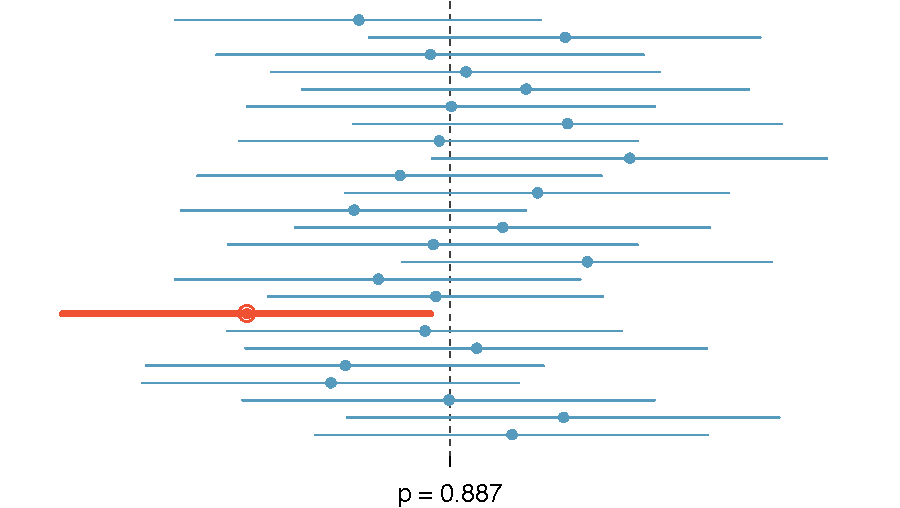
\includegraphics[width=0.75\textwidth]{ch_inference_for_props/figures/95PercentConfidenceInterval/95PercentConfidenceInterval}
   \caption{Twenty-five point estimates and confidence
       intervals from the simulations in
       Section~\ref{simulationForUnderstandingVariabilitySection}.
       For~each sample, a 95\% confidence interval was
       constructed and shown relative to the population
       proportion $p = \pewsolarpollprop{}$. Only~1 of these~25
       intervals did not capture the true population
       proportion.}
   \label{95PercentConfidenceInterval}
\end{figure}

\begin{example}{In Figure~\ref{95PercentConfidenceInterval},
one interval does not contain $p = \pewsolarpollprop{}$.
Does this imply that the population proportion cannot be
$p = \pewsolarpollprop{}$?}
Just as some observations occur more than 2 standard deviations
from the mean, some point estimates will be more than
2 standard errors from the parameter of interest.
A confidence interval only provides a plausible range
of values. While we might say other values are implausible
based on the data, this does not mean they are impossible.
\end{example}

While about 95\% of the data is within 2 standard deviations
in a normal distribution, it would be more precise to use
a value of 1.96 standard deviations. This more precise value
is typically what is used to construct confidence intervals.

\begin{termBox}{\tBoxTitle{95\% confidence interval for
    a parameter}
  When a point estimate qualifies for the Central Limit
  Theorem and closely follows a normal distribution,
  we can construct a 95\% confidence interval as
  \begin{align*}
  \text{point estimate} &\pm 1.96 \times SE
  \end{align*}}
\end{termBox}

\begin{example}{In Section~\ref{pointEstimates} we learned about
    a poll where \pewsolarpollpercent{}\% of a random sample of
    \pewsolarpollsize{} American adults
    supported expanding the role of solar power. Compute and
    interpret a 95\% confidence interval for the population
    proportion.} \label{95p_ci_for_pew_solar_support}
  We earlier confirmed that $\hat{p}$ follows a normal
  distribution and has a standard error is
  $SE_{\hat{p}} = \pewsolarpollse{}$.
  To compute the 95\% confidence interval, we plug the
  point estimate $\hat{p} = \pewsolarpollprop{}$ and
  standard error into the 95\% confidence interval formula:
  \begin{align*}
  \hat{p} \pm 1.96 \times SE_{\hat{p}}
  \quad\to\quad
  \pewsolarpollprop{} \pm 1.96 \times \pewsolarpollse{}
  \quad\to\quad
  (0.8674, 0.9066)
  \end{align*}
  We are 95\% confident that the actual proportion of
  American adults who support expanding solar power is
  between 86.74\% and 90.66\%.
\end{example}


\subsection{Changing the confidence level}
\label{changingTheConfidenceLevelSection}

\index{confidence interval!confidence level|(}

Suppose we want to consider confidence intervals where the confidence
level is somewhat higher than 95\%; perhaps we would like a confidence
level of 99\%. Think back to the analogy about trying to catch a fish:
if~we want to be more sure that we will catch the fish, we should use
a wider net. To create a 99\% confidence level, we must also widen our
95\% interval. On the other hand, if we want an interval with lower
confidence, such as 90\%, we could make our original 95\% interval
slightly slimmer.

The 95\% confidence interval structure provides guidance in how to
make intervals with new confidence levels. The general 95\% confidence
interval for a point estimate that follows the normal distribution is
normal distribution:
\begin{eqnarray}
\text{point estimate}\ \pm\ 1.96\times SE
\end{eqnarray}
There are three components to this interval: the point estimate $\hat{p}$,
``1.96'', and the standard error. The choice of $1.96\times SE$ was
based on capturing 95\% of the data since the estimate is within 1.96
standard errors of the parameter about 95\% of the time.
The choice of 1.96 corresponds to a 95\% confidence level. 

\begin{exercise} \label{leadInForMakingA99PercentCIExercise}
If $X$ is a normally distributed random variable, how often will $X$
be within 2.58 standard deviations of the mean?\footnote{This is
equivalent to asking how often the Z-score will be larger than -2.58
but less than 2.58. (For a picture, see Figure~\ref{choosingZForCI}.)
To determine this probability, we can use statistical software,
a calculator, or a table to look up -2.58 and 2.58 for the normal
distribution: 0.0049 and 0.9951. Thus, there is a
$0.9951-0.0049 \approx 0.99$ probability that an unobserved random
variable $X$ will be within 2.58 standard deviations of $\mu$.}
\end{exercise}

To create a 99\% confidence interval, change 1.96 in the 95\%
confidence interval formula to be $2.58$. Guided Practice~\ref{leadInForMakingA99PercentCIExercise} highlights
that 99\% of the time a normal random variable will be within
2.58 standard deviations of the mean. This approach -- using
the Z-scores in the normal model to compute confidence levels -- is
appropriate when $\hat{p}$ is associated with a normal distribution
with mean $p$ and standard error $SE_{\hat{p}}$. Thus, the formula
for a 99\% confidence interval for $\hat{p}$ is
\begin{eqnarray}
\hat{p}\ \pm\ 2.58\times SE_{\hat{p}}
\label{99PercCIForProp}
\end{eqnarray}

\begin{figure}
  \centering
  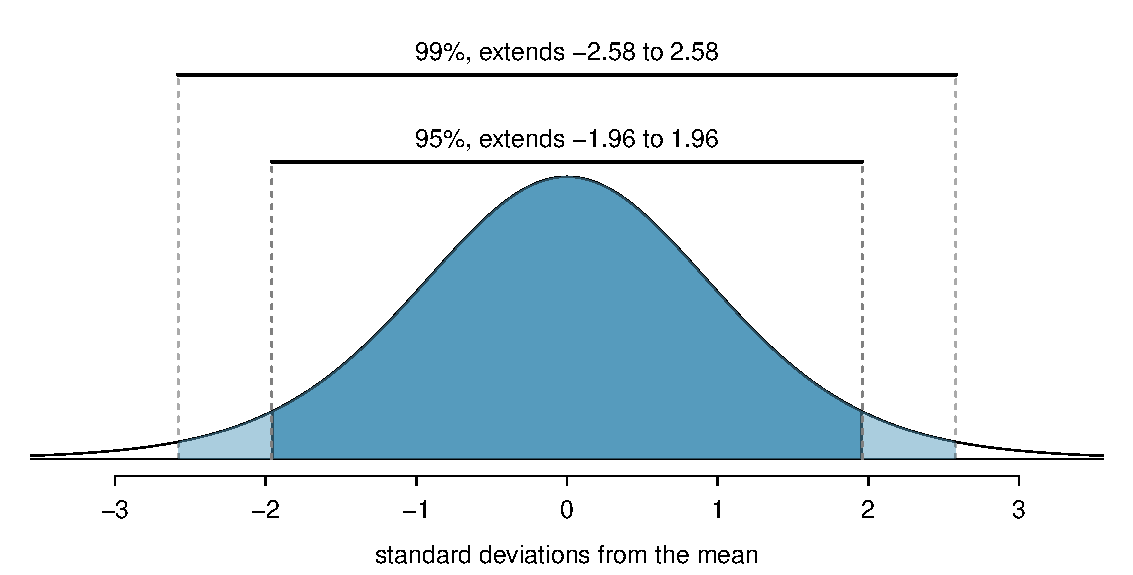
\includegraphics[width=\textwidth]{ch_inference_for_props/figures/choosingZForCI/choosingZForCI}
  \caption{The area between -$z^{\star}$ and $z^{\star}$ increases as
      $z^{\star}$ becomes larger. If the confidence level is 99\%,
      we choose $z^{\star}$ such that 99\% of the normal curve is
      between -$z^{\star}$ and $z^{\star}$, which corresponds to 0.5\%
      in the lower tail and 0.5\% in the upper tail: $z^{\star}=2.58$.}
\label{choosingZForCI}
\index{confidence interval!confidence level|)}
\end{figure}

The normal approximation is crucial to the precision of these
confidence intervals. For the context of sample proportions, the
normal distribution is reasonable to use whenever the sample
observations are independent and the success-failure condition
holds ($np$ and $n(1-p)$ are both at least 10).
For some other point estimates, the normal model is not a good fit.
In these cases, we'll use alternative distributions that better
represent the sampling distribution.

\begin{tipBox}{\tipBoxTitle[]{How to verify sample observations
    are independent}
  Subjects in an experiment are considered independent if they undergo
      random assignment to the treatment groups. \\[2mm]
  If the observations are from a simple random sample and consist
      of fewer than 10\% of the population, then they are independent.
      Even if the sample is bigger than 10\%, assuming independence
      will lead to more conservative results. \\[2mm]
  If a sample is from a seemingly random process,
      e.g. an occasional error on an assembly line,
      checking independence is more difficult. In~this case,
      use your best judgement.}
\end{tipBox}

\begin{termBox}{\tBoxTitle{Confidence interval for $p$ using any confidence level}
  If $\hat{p}$ approximately follows the normal model with
  standard error $SE_{hat{p}}$, then a confidence interval
  for the population parameter is
  \begin{eqnarray*}
  \hat{p}\ \pm\ z^{\star} SE_{\hat{p}}
  \end{eqnarray*}
  where $z^{\star}$ corresponds to the confidence level selected.}
\end{termBox}

Figure~\ref{choosingZForCI} provides a picture of how to identify
$z^{\star}$ based on a confidence level. We~select $z^{\star}$
so that the area between -$z^{\star}$ and $z^{\star}$ in the normal
model corresponds to the confidence level. 

\begin{termBox}{\tBoxTitle{Margin of error}
\label{marginOfErrorTermBox}
In a confidence interval, $z^{\star}\times SE$ is called the
\term{margin of error}.}
\end{termBox}

\begin{example}{Use the data in
    Example~\ref{95p_ci_for_pew_solar_support} to
    create a 90\% confidence interval for the proportion of American
    adults that support expanding solar power students.}
  We first find $z^{\star}$ such that 90\% of the distribution falls
  between -$z^{\star}$ and $z^{\star}$ in the standard normal model,
  $N(\mu=0, \sigma=1)$. We can do this using a graphing calculator,
  statistical software, or a probability table by looking for a lower
  tail of 5\% (the other 5\% is in the upper tail): $z^{\star}=1.65$.
  The 90\% confidence interval can then be computed as
  $\hat{p}\ \pm\ 1.65\times SE_{\hat{p}} \to (0.8705, 0.9035)$.
  (We had already verified conditions for normality and the standard error.)
  That is, we are 90\% confident that 87.1\% to 90.4\% of American
  adults support the expansion of solar power in 2018.
\end{example}



\subsection{More case studies}

\index{data!Ebola poll|(}

\newcommand{\wsjebolapollsize}{1042}
\newcommand{\wsjebolapollsizecomma}{1,042}
\newcommand{\wsjebolapollprop}{0.82}
\newcommand{\wsjebolapollpropcomplement}{0.18}
\newcommand{\wsjebolapollpercent}{82}
\newcommand{\wsjebolapollpercentcomplement}{18}
\newcommand{\wsjebolapollcount}{854}
\newcommand{\wsjebolapollcountcomplement}{188}
\newcommand{\wsjebolapollse}{0.012}


In New York City on October 23rd, 2014, a doctor who had recently been
treating Ebola patients in Guinea went to the hospital with a slight fever
and was subsequently diagnosed with Ebola. Soon thereafter,
an NBC~4 New York/The Wall Street Journal/Marist Poll found that
\wsjebolapollpercent{}\% of New Yorkers favored a ``mandatory 21-day
quarantine for anyone who has come in contact with an Ebola
patient''.\footnote{\oiRedirect{textbook-maristpoll_ebola_201410}{Poll
ID NY141026 on maristpoll.marist.edu}.} This poll included responses
of \wsjebolapollsizecomma{} New York adults between October 26th and~28th,
2014. We may want a confidence interval for the proportion of New York
adults who favored a mandatory quarantine of anyone who had been in
contact with an Ebola patient.

\begin{example}{What is the point estimate in this case,
    and is it reasonable to
    use the normal distribution to model that point estimate?}
  The point estimate, based on a sample of size $n = \wsjebolapollsize{}$,
  is $\hat{p} = \wsjebolapollprop{}$. To check whether $\hat{p}$ can be reasonably
  modeled using the normal distribution, we check independence
  (the poll is based on a simple random sample) and the
  success-failure condition
  ($\wsjebolapollsize{} \times \hat{p} \approx \wsjebolapollcount{}$
  and $\wsjebolapollsize{} \times (1 - \hat{p})
      \approx \wsjebolapollcountcomplement{}$,
  both easily greater than~10). With the conditions met, we are assured
  that the sampling distribution of $\hat{p}$ can be modeled using
  a normal distribution.
\end{example}

\begin{example}{Estimate the standard error of
    $\hat{p} = \wsjebolapollprop{}$ from the Ebola survey.}
  We'll use the substitution approximation of
  $p \approx \hat{p} = \wsjebolapollprop{}$ to compute the standard error:
  \footnote{$SE = \sqrt{\frac{p(1-p)}{n}}
    \approx \sqrt{\frac{\wsjebolapollprop{}
        (1 - \wsjebolapollprop{})}{\wsjebolapollsize{}}}
    = \wsjebolapollse{}$.}
\end{example}

\begin{example}{Construct a 95\% confidence interval for $p$,
    the proportion of New York adults who supported a quarantine
    for anyone who has come into contact with an Ebola patient.}
  Using the standard error $SE = 0.012$ from
  Example~\ref{seOfPropOfAmericansJobApprovalOfSupremeCourt},
  the point estimate \wsjebolapollprop{}, and $z^{\star} = 1.96$
  for a 95\% confidence interval, the confidence interval is
  \begin{eqnarray*}
  \text{point estimate} \ \pm\ z^{\star}SE
    \quad\to\quad \wsjebolapollprop{} \ \pm\ 1.96\times \wsjebolapollse{}
    \quad\to\quad (0.796, 0.844)
  \end{eqnarray*}
  We are 95\% confident that the proportion of New York adults
  in October 2014 who supported a quarantine for anyone who had come
  into contact with an Ebola patient was between 0.796 and 0.844.
\index{data!Ebola poll|)}
\end{example}

\begin{exercise}
Do you think the confidence interval is still valid for the opinions
of New Yorkers today?\footnote{No. The poll was taken at a
time where there was a huge public safety concern. Now that people
have had some time to step back, they may have changed their opinions.
We would need to run a new poll if we wanted to get an estimate of the
current proportion of New York adults who would support such a
quarantine period.}
\end{exercise}

\index{data!wind turbine survey|(}

\newcommand{\pewwindpollsize}{\pewsolarpollsize}
\newcommand{\pewwindpollprop}{0.848}
\newcommand{\pewwindpollpropcomplement}{0.152}
\newcommand{\pewwindpollpercent}{84.8}
\newcommand{\pewwindpollpercentcomplement}{15.2}
\newcommand{\pewwindpollcount}{848}
\newcommand{\pewwindpollcountcomplement}{152}
\newcommand{\pewwindpollse}{0.0114}

In the poll by Pew Research asking about solar energy, the
researchers also inquired about other forms of energy.
In this next case study, we examine the support for expanding wind
turbines, which received support from \pewwindpollpercent{}\%
of the \pewwindpollsize{} respondents.

\begin{exercise}\label{pew_wind_turbine_support_normal_dist_gp}
Is the normal approximation reasonable in this case?\footnote{We
check independence, which is okay since this survey was a simple
random sample, and also the success-failure condition
($\pewwindpollsize{} \times \pewwindpollprop{} = \pewwindpollcount{}$
and $\pewwindpollsize{} \times \pewwindpollpropcomplement{}
    = \pewwindpollcountcomplement$ are both at least 10).
Since both are satisfied, $\hat{p} = \pewwindpollprop{}$ can be
modeled using the normal distribution.}
\end{exercise}

\begin{exercise}
Using the Pew Research survey where $n = \pewwindpollsize{}$ and
$\hat{p} = \pewwindpollprop{}$, create a 99\% confidence interval
for the level of American support for expanding the use of wind
turbines for power
generation.\footnote{Guided
Practice~\ref{pew_wind_turbine_support_normal_dist_gp}
confirmed that that $\hat{p}$ closely follows a normal distribution,
so we can use the confidence interval formula:
\begin{align*}
\text{point estimate} \pm z^{\star} SE
\end{align*}
In this case, the point estimate is $\hat{p} = \pewwindpollprop{}$.
For a 99\% confidence interval, $z^{\star} = 2.58$. Computing the
standard error:
$SE_{\hat{p}}
  = \sqrt{\frac{\pewwindpollprop{}(1 - \pewwindpollprop{})}
      {\pewwindpollsize{}}}
  = \pewwindpollse{}$.
Finally, we compute the interval as
$\pewwindpollprop{} \pm 2.58 \times \pewwindpollse{} \to (0.8186, 0.8774)$.
It is also \emph{always} important to provide an interpretation for
the interval: we are 99\% confident the proportion of
Americans adults that support expanding the use of wind
turbines is between 81.9\% and 87.7\% in 2018.}
\end{exercise}




\subsection{Interpreting confidence intervals}
\label{interpretingCIs}

\index{confidence interval!interpretation|(}

In each of the examples, we described the confidence
intervals by putting them into the context of the data and also
using somewhat formal language:
\begin{description}
  \item[Solar.] We are 90\% confident that 87.1\% to 90.4\% of
      American adults support the expansion of solar power in 2018.
  \item[Ebola.] We are 95\% confident that the proportion
      of New York adults in October 2014 who supported a quarantine
      for anyone who had come into contact with an Ebola patient was
      between 0.796 and 0.844.
  \item[Wind Turbine.] We are 99\% confident the proportion of
      Americans adults that support expanding the use of wind
      turbines is between 81.9\% and 87.7\% in 2018.
\end{description}
First, notice that the statements are always about the population
parameter, which considers all American adults for the energy polls
and all New York adults for the quarantine poll, \emph{not} only
the adults included in the sample.

We also avoided another common mistake:
\emph{incorrect} language might try to describe the confidence interval
as capturing the population parameter with a certain probability.
Making a probability interpretation is a common error:
while it might be useful to think of it as a probability,
the confidence level only quantifies how plausible
it is that the parameter is in the interval.

Another important consideration of confidence intervals is that they
\emph{only try to capture the population parameter}. A confidence
interval says nothing about the confidence of capturing individual
observations, a proportion of the observations, or about capturing
point estimates. Confidence intervals only attempt to capture
population parameters.

\index{data!wind turbine survey|)}
\index{data!solar survey|)}
\index{confidence interval!interpretation|)}

\CalculatorVideos{confidence intervals for a single proportion}

\index{confidence interval|)}




%__________________
%\section[Hypothesis testing]{Hypothesis testing \sectionvideohref{youtube-NVbPE1_Cbx8&list=PLkIselvEzpM7Pjo94m1e7J5jkIZkbQAl4}~\sectionslideshref{gdoc_os3_slides_4-3}}
\section{Hypothesis testing for a proportion}
\label{hypothesis_testing_one_prop}
\label{hypothesisTesting}

\index{hypothesis testing|(}

Warren Buffett is a legendary investor who has made a fortune
of about \$85~billion in the stock market. His net worth is
more than the gross domestic product of dozens of countries.
As perhaps the most thoughtful investors of our time, Buffett
has advised people to steer clear of hedge funds and instead
invest directly in an index
fund.\footnote{\oiRedirect{buffett-invest-in-index-fund}{www.cnbc.com/2018/01/03/why-warren-buffett-says-index-funds-are-the-best-investment.html}}
\Comment{Make sure the URL link goes where it should.}

Buffett's suggestion is that hedge funds tend to give lower
rates of return than index funds, and it is helpful to test
that theory! We'll look at a sample of managed funds
and see whether these funds tend to beat or fall behind a
standard index fund.






%There's an adage in United States financial markets that
%it is better to get out of investments during the six ``summer''
%months: \emph{sell in May and go away!}\footnote{Summer in the
%northern hemisphere, anyways. \rotatebox[origin=c]{180}{(Hello
%Australia!)}} While this clever saying does rhyme, that doesn't
%mean it is sound financial advice. Let's investigate.

%so is this is a pretty strong statement, since the stock
%market has a very strong historical trend of moving upwards.
%
%To test this theory, we've retrieved the 
%
%If this adage holds meaning, we would expect that about half of the time the market would be in decline each year. Of course, we also would care to learn if it happens to be up more often than not, so we will also check that!

%Finance is a field where a lot of money can be made or lost. We're going to explore a few topics in relation to the US stock market and 

%The United States stock market moves down and up in unpredictable ways, and it can be useful to look for small inconsistencies in the market behavior that can be leveraged for minor gains. We will test three theories about the stock market in this section:

%\item We might wonder whether the stock market is more likely to go up or down in any given day. Of course, the average return each day has been historically positive, and so this exploration will allow us to better understand if that is also reflected in the fraction of days that are up.
%\item Each week there is a 65.5 hours window from the time the market closes on Friday to when it opens on the weekdays. That's a lot of time for good news and bad news that can affect the returns on Mondays. We'll see whether we 

%The market has the same chance of going up or down on any given day of the week. For example, we would be interested to learn if the stock market goes up a little more often on, say, Fridays, that could be useful for 


\subsection{Hypothesis testing framework}

%We took a sample of 50 actively managed funds in the
%United States and compared their performance to that of the
%S\&P 500 stock index. 
%
%Ultimately, we want to understand: which
%has a better chance of outperforming the other, the actively
%managed fund or the index fund?
%The data for this study can be found in \data{active_fund},
%and it is summarized in Table~\ref{}

\Comment{When reviewing, make the discussion more clearly focused on the proportion of fund managers that beat the index fund.}

The historical return rate in the stock market is about 7\%.
Many fund managers believe their knowledge about the market gives
them a leg up and that they can get a higher return. While
they may invest their own money, these fund managers
find investors who are willing to bet on their skills,
and for their trouble they get a cut any financial
gains.\footnote{Getting even just an 8\% return over a 7\%
return would be hugely valuable, since the gains compound over
time. For example, \$1000 invested at 7\% will be be about
\$7600 after 30 years while it would have been \$10,000 with
an 8\% return.}

We all would like to know: what fraction of fund managers
outperform a simple index fund? We'll be using the S\&P~500
index fund as our source of comparison.
Ultimately, there are two possibilities:
\begin{description}
\item[$H_0$:] %$\mathbf{H_0}$: Even chance of beating S\&P~500.]
  If we randomly picked a fund manager, there's a 50-50 chance
  they'll beat the S\&P~500.
\item[$H_A$:] %$\mathbf{H_A}$: Either fund managers or the S\&P~500 is better.]
  There's something more systematic: the proportion of fund
  managers who beat the S\&P~500 isn't 50\%. That is, the
  proportion is either less than 50\% or greater than 50\%.
%  That is, it is  fund managers or the S\&P~500 is better.
%  That said, we're not sure which it will be!
%  While we don't know which will do better, we 
%  We aren't sure which it might be, but one of
%  these investment approaches is typically better than the
%  other.
\end{description}
%Ultimately, we don't know which is true!
These competing ideas are called \term{hypotheses}.
We call $H_0$ the null hypothesis and $H_A$ the alternative
hypothesis.

\begin{termBox}{\tBoxTitle{Null and alternative hypotheses}
  The \term{null hypothesis ($H_0$)} often represents
  either a skeptical perspective or a claim to be tested.
  The \term{alternative hypothesis ($H_A$)} represents an
  alternative claim under consideration and is often
  represented by a range of possible parameter values.}
\end{termBox}

The null hypothesis often represents a skeptical position
or a perspective of no difference. This makes sense for our
setup with the fund managers: we're basically saying that
there's no difference and it's a flip of the coin on whether
a fund manager beats the S\&P~500.

The alternative hypothesis generally represents a new
or stronger perspective. In the case of the fund managers,
it would certainly be interesting to learn whether most fund
managers beat the S\&P~500 index fund, since that would mean
there are potential benefits to working with the typical fund
manager. It would also be darn interesting if it were true
that most fund managers don't beat the index fund, since
that would mean the typical fund manager is effectively paid
to \emph{lose} the money for their investors!

\begin{tipBox}{\tipBoxTitle{Be a skeptic of $\mathbf{H_A}$
    and require supporting evidence}
  The alternative hypothesis is generally an assertion of
  something genuinely interesting or new. For this reason,
  our job as data scientists is to play the role of a skeptic:
  before we buy into the alternative hypothesis, we need to
  see strong supporting evidence.}
\end{tipBox}

The hypothesis testing framework is a very general tool, and we often use it without a second thought. If a person makes a somewhat unbelievable claim, we are initially skeptical. However, if there is sufficient evidence that supports the claim, we set aside our skepticism and reject the null hypothesis in favor of the alternative. The hallmarks of hypothesis testing are also found in the US court system. 

\begin{exercise} \label{hypTestCourtExample}
A US court considers two possible claims about a defendant: she is either innocent or guilty. If we set these claims up in a hypothesis framework, which would be the null hypothesis and which the alternative?\footnote{The jury considers whether the evidence is so convincing (strong) that there is no reasonable doubt regarding the person's guilt; in such a case, the jury rejects innocence (the null hypothesis) and concludes the defendant is guilty (alternative hypothesis).}
\end{exercise}

\begin{tipBox}{\tipBoxTitle{Double negatives can sometimes be used in statistics}
In many statistical explanations, we use double negatives. For instance, we might say that the null hypothesis is \emph{not implausible} or we \emph{failed to reject} the null hypothesis. Double negatives are used to communicate that while we are not rejecting a position, we are also not saying it is correct.}
\end{tipBox}

Jurors examine the evidence to see whether it convincingly shows a defendant is guilty. Even if the jurors leave unconvinced of guilt beyond a reasonable doubt, this does not mean they believe the defendant is innocent. This is also the case with hypothesis testing: \emph{even if we fail to reject the null hypothesis, we typically do not accept the null hypothesis as true}. Failing to find strong evidence for the alternative hypothesis is not equivalent to accepting the null hypothesis.

In the fund manager example, the null hypothesis represents
the notion that it's a flip of the coin whether any given
fund manager will beat the S\&P~500. That is, the proportion
$p$ of fund managers who beat the S\&P~500 is 50\%.
The alternative hypothesis is that this proportion is something
other than 50\%. While it's helpful to write these hypotheses
in words, it can be simpler to write them using mathematical
notation:
\begin{description}
\item[$H_0$:] $p = 0.50$
\item[$H_A$:] $p \neq 0.50$
\end{description}
In this hypothesis setup, we want to make a conclusion about
the population parameter $p$. The value we are comparing the
parameter to is called the \term{null value}, which in this
case is 0.50. It's common to label the null value with the
same symbol as the parameter but with a subscript `0'.
That is, in this case, the null value is $p_0 = 0.50$.

\begin{example}{It may seem impossible that the
    proportion of fund managers that beat the S\&P~500
    is \emph{exactly} 50\%. If we don't believe the
    null hypothesis, should we simply reject it?}
  \label{fund_managers_sp500_not_reject_H0_interpretation}
  No. While we may not buy into the notion that
  the proportion is exactly 50\%, the hypothesis testing
  framework requires that there be strong evidence before
  we reject the null hypothesis and conclude something
  more interesting.

  After all, even if we don't believe the proportion is
  \emph{exactly} 50\%, that doesn't really tell us anything
  useful! We would still be stuck with the original question:
  do fund managers tend to beat the S\&P~500 or vice-versa?
  Without data that strongly
  points in one direction or the other, it is entirely
  uninteresting and pointless to reject $H_0$.
\end{example}

\begin{exercise}
  Another hypothesis test might be testing whether a new drug
  is better or worse than an existing drug at treating headaches.
  What should we use for the null and alternative hypotheses in
  this case?\footnote{The null hypothesis ($H_0$) in this case
  is the declaration of \emph{no difference}: the drugs are equally
  effective. The alternative hypothesis ($H_A$).}
\end{exercise}
  
%Suppose we collected data but the data didn't show strong
%evidence that the new drug performs better or worse than the
%old drug. That doesn't mean the new drugs have the exact same
%effectiveness. However, that does not mean the drugs perform
%equally; it may be that we simply were unable to detect which
%drug was in fact better than the other.






\subsection{Testing hypotheses using confidence intervals}
\label{utilizingOurCI}

\Comment{Build the \data{fund\_managers} data set and put it
in the R package. Only considering large-cap fund managers.
See \href{https://us.spindices.com/documents/spiva/spiva-us-year-end-2016.pdf}{this report} as a reference.}

We will use the \data{fund\_managers} data set to evaluate
the hypothesis test evaluating whether the proportion of fund
managers who beat the S\&P~500 is different from 50\%. This
data set summarizes the performance of 100 randomly sampled
fund managers during the 2016 and evaluates whether each
beat the S\&P~500 or not. Of those 100 managers,
$\hat{p} = 0.36$ (36\%) beat the S\&P~500 while the other
54\% did not.

Up until now, our discussion has been philosophical.
However, now that we have data, we might ask ourselves:
does the data provide strong evidence that the proportion
of all fund managers is different than 50\%?

We learned in Section~\ref{pointEstimates} that there is
fluctuation from one sample to another, and it is unlikely
that $\hat{p}$ will exactly equal $p$, and we want to make
a conclusion about $p$. So we are still left with a nagging
concern: is this deviation of 36\% from 50\% simply due to
chance, or does the data provide strong evidence that the
true proportion is different from 50\%?

In Section~\ref{confidenceIntervals}, we learned how to
quantify the uncertainty in our estimate using confidence
intervals. This can be useful for the hypothesis test.

\begin{example}{Check whether it is reasonable to construct
    a confidence interval for $p$ using the sample data, and
    if so, construct a 95\% confidence interval. Also use
    the confidence interval to evaluate the hypothesis test.}
  The conditions are met for $\hat{p}$ to be approximately
  normal: the data come a simple random sample (satisfies
  independence), and $n\hat{p} = 36$ and
  $n(1 - \hat{p}) = 64$ are both greater than 10 (success-failure
  condition).

  To construct the confidence interval, we will need to identify
  the point estimate ($\hat{p} = 0.36$), the critical value for
  the 95\% confidence level ($z^{\star} = 1.96$), and the standard
  error of $\hat{p}$
  ($SE_{\hat{p}} = \sqrt{\hat{p}(1 - \hat{p}) / n} = 0.048$).
  With those items, we can construct a confidence interval for $p$:
  \begin{align*}
    &\hat{p} \pm z^{\star} \times SE_{\hat{p}} \\
    &0.36 \pm 1.96 \times 0.048 \\
    &(0.266, 0.454)
  \end{align*}
  We are 95\% confident that the proportion of all fund
  managers who beat the S\&P~500 in 2016 was between 26.6\%
  and 45.4\%.

  The confidence interval falls entirely below the
  null value, $p_0 = 0.50$, which gives us strong evidence
  that the proportion is in fact not 50\%.
  More importantly,
  the confidence interval provides strong evidence that the
  actual proportion of fund managers who beat the S\&P~500
  is below 50\%.\footnote{You might be asking
  yourself whether there was something special about 2016;
  perhaps the fund managers perform better in other years.
  If this question came to mind, then great job on being
  a skeptic! This is an important question to ask,
  and we looked at research on the topic:
  the 2016 finding is consistent with other historical data.
  For example, when tracking a 15-year period ending
  in 2016, only about 8\% of fund managers beat the S\&P~500:
  \oiRedirect{sp500-beats-fund-managers-report}{us.spindices.com/documents/spiva/spiva-us-year-end-2016.pdf}}
  \Comment{Ensure the redirect in the footnote works.}
\end{example}
%At a first glance, it looks like it might be. After all,
%36\% isn't that close to 50\%, so maybe this data constitutes
%\emph{strong evidence}. We need to 

Had the confidence interval contained the null value,
in this case $p_0 = 0.5$, then the data would have been
insufficient evidence to reject the null hypothesis.
That is, had that been the case, the null value would
have been in the \emph{range of plausible values}
(at the 95\% confidence level), so we would not have
had sufficient evidence to reject the notion that the
proportion was actually 0.5.
As discussed in
Example~\ref{fund_managers_sp500_not_reject_H0_interpretation},
failing to reject the
null hypothesis does not necessarily mean we believe
it is true, but it does mean we cannot conclude anything
interesting (e.g. cannot differentiate whether the
the proportion of fund managers that provides a better
return on investment than index funds is smaller or
larger than 0.5.

%You might wonder about what would happen if we had used
%a higher confidence level, such as 99\% or 99.9\%. If we
%use a high enough confidence level, the interval will end
%up being wide enough.

\Comment{Introduce and go through a second case study.}



\subsection{Decision errors}

\index{hypothesis testing!decision errors|(}

Hypothesis tests are not flawless, since we can make a wrong decision in statistical hypothesis tests based on the data. For example, in the court system innocent people are sometimes wrongly convicted and the guilty sometimes walk free. However, the difference is that in statistical hypothesis tests, we have the tools necessary to quantify how often we make such errors.

% Hypothesis tests are not flawless. Just think of the court system: innocent people are sometimes wrongly convicted and the guilty sometimes walk free. Similarly, we can make a wrong decision in statistical hypothesis tests. However, the difference is that we have the tools necessary to quantify how often we make such errors.

There are two competing hypotheses: the null and the alternative. In a hypothesis test, we make a statement about which one might be true, but we might choose incorrectly. There are four possible scenarios, which are summarized in Table~\ref{fourHTScenarios}.

\begin{table}[ht]
\centering
\begin{tabular}{l l c c}
& & \multicolumn{2}{c}{\textbf{Test conclusion}} \\
  \cline{3-4}
\vspace{-3.7mm} \\
& & do not reject $H_0$ &  reject $H_0$ in favor of $H_A$ \\
  \cline{2-4}
\vspace{-3.7mm} \\
& $H_0$ true & okay &  Type~1 Error \\
\raisebox{1.5ex}{\textbf{Truth}} & $H_A$ true & Type~2 Error & okay \\
  \cline{2-4}
\end{tabular}
\caption{Four different scenarios for hypothesis tests.}
\label{fourHTScenarios}
\end{table}

A \term{Type~1 Error} is rejecting the null hypothesis when $H_0$ is actually true. A \term{Type~2 Error} is failing to reject the null hypothesis when the alternative is actually true.

\begin{exercise} \label{whatAreTheErrorTypesInUSCourts}
In a US court, the defendant is either innocent ($H_0$) or  guilty ($H_A$). What does a Type~1 Error represent in this context? What does a Type~2 Error represent? Table~\ref{fourHTScenarios} may be useful.\footnote{If the court makes a Type~1 Error, this means the defendant is innocent ($H_0$ true) but wrongly convicted. A Type~2 Error means the court failed to reject $H_0$ (i.e. failed to convict the person) when she was in fact guilty ($H_A$ true).}
\end{exercise}

\begin{exercise} \label{howToReduceType1ErrorsInUSCourts}
How could we reduce the Type~1 Error rate in US courts? What influence would this have on the Type~2 Error rate?\footnote{To lower the Type~1 Error rate, we might raise our standard for conviction from ``beyond a reasonable doubt'' to ``beyond a conceivable doubt'' so fewer people would be wrongly convicted. However, this would also make it more difficult to convict the people who are actually guilty, so we would make more Type~2 Errors.}
\end{exercise}

\begin{exercise} \label{howToReduceType2ErrorsInUSCourts}
How could we reduce the Type~2 Error rate in US courts? What influence would this have on the Type~1 Error rate?\footnote{To lower the Type~2 Error rate, we want to convict more guilty people. We could lower the standards for conviction from ``beyond a reasonable doubt'' to ``beyond a little doubt''. Lowering the bar for guilt will also result in more wrongful convictions, raising the Type~1 Error rate.}
\end{exercise}

\index{hypothesis testing!decision errors|)}

Exercises~\ref{whatAreTheErrorTypesInUSCourts}-\ref{howToReduceType2ErrorsInUSCourts} provide an important lesson: if we reduce how often we make one type of error, we generally make more of the other type.

Hypothesis testing is built around rejecting or failing to reject the null hypothesis. That is, we do not reject $H_0$ unless we have strong evidence. But what precisely does \emph{strong evidence} mean? As a general rule of thumb, for those cases where the null hypothesis is actually true, we do not want to incorrectly reject $H_0$ more than 5\% of the time. This corresponds to a \term{significance level}\index{hypothesis testing!significance level} of 0.05. We often write the significance level using $\alpha$ (the Greek letter \emph{alpha}\index{Greek!alpha@alpha ($\alpha$)}): $\alpha = 0.05$. We discuss the appropriateness of different significance levels in Section~\ref{significanceLevel}. \Comment{Get this ref is working.}

If we use a 95\% confidence interval to evaluate a hypothesis test where the null hypothesis is true, we will make an error whenever the point estimate is at least 1.96 standard errors away from the population parameter. This happens about 5\% of the time (2.5\% in each tail). Similarly, using a 99\% confidence interval to evaluate a hypothesis is equivalent to a significance level of $\alpha = 0.01$.

A confidence interval is, in one sense, simplistic in the world of hypothesis tests. Consider the following two scenarios:
\begin{itemize}
\setlength{\itemsep}{0mm}
\item The null value (the parameter value under the null hypothesis) is in the 95\% confidence interval but just barely, so we would not reject $H_0$. However, we might like to somehow say, quantitatively, that it was a close decision.
\item The null value is very far outside of the interval, so we reject $H_0$. However, we want to communicate that, not only did we reject the null hypothesis, but it wasn't even close. Such a case is depicted in Figure~\ref{whyWeWantPValue}.
\end{itemize}
In Section~\ref{pValue}, we introduce a tool called the \emph{p-value} that will be helpful in these cases. The p-value method also extends to hypothesis tests where confidence intervals cannot be easily constructed or applied.

\begin{figure}[hht]
\centering
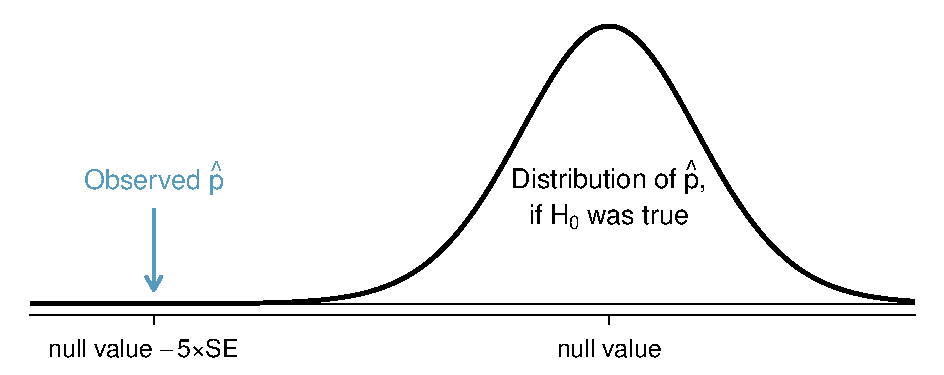
\includegraphics[width=0.75\textwidth]{ch_inference_for_props/figures/whyWeWantPValue/whyWeWantPValueProp}
\caption{It would be helpful to quantify the strength of the evidence against the null hypothesis. In this case, the evidence is extremely strong.}
\label{whyWeWantPValue}
\end{figure}



\subsection{Formal testing using p-values}

\label{pValue}

\index{hypothesis testing!p-value|(}

The p-value is a way of quantifying the strength of the evidence against the null hypothesis and in favor of the alternative. Formally the \emph{p-value} is a conditional probability.

\begin{termBox}{\tBoxTitle{p-value}
The \term{p-value}\index{hypothesis testing!p-value|textbf} is the probability of observing data at least as favorable to the alternative hypothesis as our current data set, if the null hypothesis is true. We typically use a summary statistic of the data, in this section the sample proportion, to help compute the p-value and evaluate the hypotheses.}
\end{termBox}

Statistical hypothesis testing almost always uses the p-value method rather than confidence intervals. In this formal space of hypothesis testing for proportions, we will slightly modify how we check the success-failure condition and compute the standard error. These changes aren't dramatic, but they will require paying a little more attention to how we use the null value, $p_0$.

%To apply the normal distribution framework in the context of a hypothesis test for a proportion, the independence and success-failure conditions must be satisfied. In a hypothesis test, the success-failure condition is checked using the null proportion: we verify $np_0$ and $n(1-p_0)$ are at least 10, where $p_0$ is the null value.

\index{data!coal power support|(}

\begin{example}{Pew Research asked a random sample of 1000 American
    adults whether they supported the increased usage of
    coal. Set up hypotheses to evaluate whether this represents
    a majority of Americans, one way or the other.}
  The uninteresting result is that there is no majority either way:
  half of Americans support and the other half oppose expanding the
  use of coal to produce energy. The alternative hypothesis would
  be that there is a majority support (or oppose) to expanding the
  use of coal. If $p$ represents the proportion supporting, then
  we can write the hypotheses as
  \begin{description}
    \item[$H_0$:] $p = 0.5$
    \item[$H_A$:] $p \neq 0.5$
  \end{description}
  In this case, the null value ($p_0$) is 0.5.
\end{example}

Pew Research's sample found that 37\% of American adults support
increased usage of coal. We now wonder, does 37\% represent a
real difference from the null hypothesis of 50\%.

\begin{example}{What would the sampling distribution of $\hat{p}$
    look like if the null hypothesis were true?}
  If the null hypothesis were true, the population proportion
  would be the null value, 0.5. We previously learned that
  the sampling distribution of $\hat{p}$ will be normal when
  two conditions are met:
  \begin{itemize}
    \item Independence is reasonable since this poll is based on
        a simple random sample.
    \item Based on the poll's sample size of $n = 1000$,
        the success-failure condition is met, since
        \begin{align*}
        np \quad \stackrel{H_0}{=} \quad 1000 \times 0.5 = 500
        \qquad
        n (1 - p) \quad \stackrel{H_0}{=} \quad 1000 \times (1 - 0.5) = 500
        \end{align*}
        are both greater than 10. Note that the success-failure
        condition was checked using the null value, $p_0 = 0.5$;
        this is the first procedural difference from confidence
        intervals.
  \end{itemize}
  If the null hypothesis were true, the sampling distribution
  indicates that a sample proportion based on $n = 1000$ observations
  would be normally distributed. Next, we can compute the standard
  error, where we will again use the null value $p_0 = 0.5$ in the
  calculation:
  \begin{align*}
  SE = \sqrt{\frac{p (1 - p)}{n}}
      \quad \stackrel{H_0}{=} \quad \sqrt{\frac{0.5 \times 0.5}{1000}}
      = 0.016
  \end{align*}
  This marks the other procedural difference from confidence
  intervals: since the sampling distribution is determined
  under the null proportion, the null value $p_0$ was used for
  the proportion in the calculation rather than $\hat{p}$.

  Ultimately, if the null hypothesis were true, then the sample
  proportion should follow a normal distribution with mean 0.500
  and standard error of 0.016. This distribution is shown in
  Figure~\ref{normal_dist_mean_500_se_016}.
\end{example}

\begin{figure}[hht]
\centering
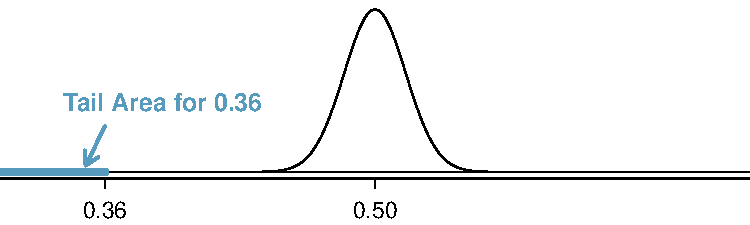
\includegraphics[width=0.75\textwidth]{ch_inference_for_props/figures/normal_dist_mean_500_se_016/normal_dist_mean_500_se_016}
\caption{
  If the null hypothesis were true, this normal distribution
  describes the distribution of $\hat{p}$. It appears that,
  if $H_0$ were true, then it is very unlikely to observe
  $\hat{p} = 0.36$. To say how unlikely, we use the tail area.}
\label{normal_dist_mean_500_se_016}
\end{figure}


When we identify the sampling distribution under the null hypothesis,
it has a special name: the \term{null distribution}. The p-value
represents the probability of the observed $\hat{p}$, or a $\hat{p}$
that is more extreme, if the null hypothesis were true.

\begin{example}{Compute the chance that $\hat{p} = 0.36$ or
    further from 0.5 under the null distribution, which is a
    normal distribution with mean 0.5 and $SE = 0.016$.}
  This is a normal probability problem where $x = 0.36$.
  First, we draw a simple graph to represent the situation,
  similar to what is shown in
  Figure~\ref{normal_dist_mean_500_se_016}.
  Since $\hat{p}$ is so far out in the tail, we know the
  tail area is going to be very small. To find it, we start
  by computing the Z-score using the mean of 0.5 and the
  standard error of 0.016:
  \begin{align*}
  Z = \frac{0.37 - 0.5}{0.016} = 8.125 
  \end{align*}
  We can use the normal probability table or software to find
  the tail area. If we use the probability table, we consider the
  smallest Z-score shown, which in
  Appendix~\ref{normalProbabilityTable}
  corresponds to a tail area of 0.0002.

  To get the p-value, we double this tail area, since observations
  in the mirror-imaged tail
  (Figure~\ref{normal_dist_mean_500_se_016_with_upper})
  are also just as extreme
  relative to 0.5 as those below 0.36.
  This gives a p-value of 0.0004.

  Here, the p-value represents the probability of observing
  such an extreme sample proportion by chance, if the null hypothesis
  were true.
\end{example}

\begin{figure}[hht]
\centering
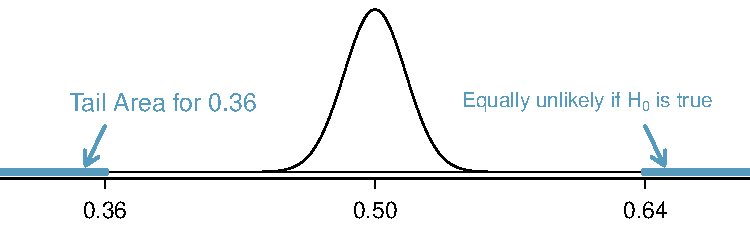
\includegraphics[width=0.75\textwidth]{ch_inference_for_props/figures/normal_dist_mean_500_se_016/normal_dist_mean_500_se_016_with_upper}
\caption{
  If $H_0$ were true, then the values above 0.64 are just
  as unlikely as values below 0.36.}
  %, so we double the lower
  %tail to get the p-value. This represents the probability
  %of observing something at least as extreme as
  %$\hat{p} = 0.36$, if the null hypothesis were true.}
\label{normal_dist_mean_500_se_016_with_upper}
\end{figure}




\begin{example}{How should we evaluate the hypotheses using the
    p-value of 0.0004? Use the standard significance level of
    $\alpha = 0.05$.}
  If the null hypothesis were true, it's very unlikely that we would
  observe such an extreme deviation of $\hat{p}$ from 0.5. This means
  there are one of two possibilities:
  \begin{enumerate}
    \item The null hypothesis is true, and we just happened to get
        really unlucky.
    \item The alternative hypothesis is true, which would be consistent
        with observing a sample proportion far from 0.5.
  \end{enumerate}
  The p-value tells us that what we observed is so unusual
  with respect to null hypothesis that it casts serious doubt on $H_0$.
  Formally, we compare the p-value to the significance level
  $\alpha = 0.05$. Since the p-value is less than $\alpha$,
  we reject the null hypothesis.
  That is, the data provide strong evidence against $H_0$,
  and we conclude that a majority of Americans do not support
  expanding the use of coal.
\end{example}

\index{data!coal power support|)}

\begin{tipBox}{
  \tipBoxTitle{Compare the p-value to $\mathbf{\alpha}$ to
      evaluate $\mathbf{H_0}$}
  When the p-value is less than the significance level, $\alpha$,
  reject $H_0$. We would report a conclusion that the data provide
  strong evidence supporting the alternative hypothesis. \\[2mm]
  When the p-value is greater than $\alpha$, do not reject $H_0$,
  and report that we do not have sufficient evidence to reject the
  null hypothesis. \\[2mm]
  In either case, it is important to describe the conclusion
  in the context of the data.}
\end{tipBox}







\index{data!nuclear arms reduction|(}

\begin{exercise}
Do a majority of American support or oppose nuclear arms reduction? Set up hypotheses to evaluate this question.\footnote{We would like to understand if a majority supports or opposes, or ultimately, if there is no difference. $H_0: p = 0.50$. $H_A: p > 0.50$.}
\end{exercise}

\begin{example}{A simple random sample of 1,028 US adults in March 2013 found that 56\% support nuclear arms reduction.\footnote{\oiRedirect{textbook-nuclear_arms_reduction_201303}{www.gallup.com/poll/161198/favor-russian-nuclear-arms-reductions.aspx}} Does this provide convincing evidence that a majority of Americans supported nuclear arms reduction at the 5\% significance level?} \label{NuclearArmsInferenceExample}
The poll was of a simple random sample that includes fewer than 10\% of US adults, meaning the observations are independent. In a one-proportion hypothesis test, the success-failure condition is checked using the null proportion, which is $p_0 = 0.5$ in this context: $n p_0 = n (1 - p_0) = 1028 \times 0.5 = 514 > 10$. With these conditions verified, the normal model may be applied to $\hat{p}$.

Next the standard error can be computed. The null value $p_0$ is used again here, because this is a hypothesis test for a single proportion.
\begin{align*}
SE = \sqrt{\frac{p_0 (1 - p_0)}{n}} = \sqrt{\frac{0.5 (1 - 0.5)}{1028}} = 0.016
\end{align*}
A picture of the normal model is shown in Figure~\ref{nuclearArmsReductionPValue} with the p-value represented by the shaded region. Based on the normal model, the test statistic can be computed as the Z-score of the point estimate:
\begin{align*}
Z = \frac{\text{point estimate} - \text{null value}}{SE} = \frac{0.56 - 0.50}{0.016} = 3.75
\end{align*}
The upper tail area, representing the p-value, is about 0.0001. Because the p-value is smaller than 0.05, we reject $H_0$. The poll provides convincing evidence that a majority of Americans supported nuclear arms reduction efforts in March 2013.
\end{example}

\begin{figure}[h]
\centering
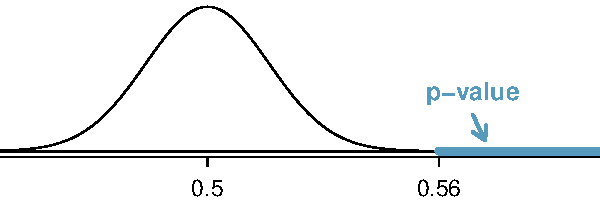
\includegraphics[width=0.48\textwidth]{ch_inference_for_props/figures/nuclearArmsReduction/nuclearArmsReductionPValue}
\caption{Sampling distribution for Example~\ref{NuclearArmsInferenceExample}.}
\label{nuclearArmsReductionPValue}
\end{figure}

\begin{termBox}{\tBoxTitle{Hypothesis testing steps for a proportion}
Once you've determined a one-proportion hypothesis test is the
correct procedure, there are four steps to completing the
test:
\begin{description}
\item[Choose.] Identify the parameter of interest,
    select the method to apply
    (e.g. confidence interval or hypothesis test),
    list out hypotheses,
    identify $\hat{p}$ and $n$.
\item[Check.] Verify the conditions using the null value,
    $p_0$, to ensure $\hat{p}$ is nearly normal under $H_0$.
\item[Calculate.] If the conditions hold, compute the standard
    error, again using $p_0$, and identify the p-value.
\item[Conclude.] Evaluate the hypotheses by comparing the p-value
    to $\alpha$, and provide a conclusion in the context of the
    problem.
\end{description}}
\end{termBox}

\index{data!nuclear arms reduction|)}

%\begin{termBox}{\tBoxTitle{p-value as a tool in hypothesis testing}
%The smaller the p-value, the stronger the data favor $H_A$ over $H_0$. A small p-value (usually $<0.05$) corresponds to sufficient evidence to reject $H_0$ in favor of $H_A$.}
%\index{hypothesis testing!p-value|)}
%\end{termBox}

%\begin{tipBox}{\tipBoxTitle{It is useful to first draw a picture to find the p-value}
%It is useful to draw a picture of the distribution of $\bar{x}$ as though $H_0$ was true (i.e.~$\mu$~equals the null value), and shade the region (or regions) of sample means that are at least as favorable to the alternative hypothesis. These shaded regions represent the p-value.}
%\end{tipBox}

\CalculatorVideos{hypothesis tests for a single proportion}



\subsection{Choosing a significance level}
\label{significanceLevel}

\index{hypothesis testing!significance level|(}
\index{significance level|(}

Choosing a significance level for a test is important in
many contexts, and the traditional level is $\alpha = 0.05$.
However, it's often helpful to adjust the significance level
based on the application. We may select a level that is
smaller or larger than 0.05 depending on the consequences
of any conclusions reached from the test.

If making a Type~1 Error is dangerous or especially costly,
we should choose a small significance level (e.g. 0.01).
Under this scenario we want to be very cautious about
rejecting the null hypothesis, so we demand very strong
evidence favoring $H_A$ before we would reject $H_0$.

If a Type~2 Error is relatively more dangerous or much more
costly than a Type~1 Error, then we should choose a higher
significance level (e.g. 0.10). Here we want to be cautious
about failing to reject $H_0$ when the null is actually false.

\begin{tipBox}{\tipBoxTitle[]{Significance levels should
    reflect consequences of errors}
  The significance level selected for a test should reflect
  the consequences associated with Type~1 and Type~2 Errors.}
\end{tipBox}

\begin{example}{A car manufacturer is considering a higher
    quality but more expensive supplier for window parts in
    its vehicles. They sample a number of parts from their
    current supplier and also parts from the new supplier.
    They decide that if the high quality parts will last
    more than 12\% longer, it makes financial sense to
    switch to this more expensive supplier. Is there good
    reason to modify the significance level in such a
    hypothesis test?}
  The null hypothesis is that the more expensive parts last
  no more than 12\% longer while the alternative is that they
  do last more than 12\% longer. This decision is just one of
  the many regular factors that have a marginal impact on the
  car and company. A significance level of 0.05 seems
  reasonable since neither a Type~1 or Type~2 Error should
  be dangerous or (relatively) much more expensive.
\end{example}

\begin{example}{The same car manufacturer is considering
    a slightly more expensive supplier for parts related
    to safety, not windows. If the durability of these
    safety components is shown to be better than the
    current supplier, they will switch manufacturers.
    Is there good reason to modify the significance level
    in such an evaluation?}
  The null hypothesis would be that the suppliers' parts
  are equally reliable. Because safety is involved,
  the car company should be eager to switch to the slightly
  more expensive manufacturer (reject $H_0$) even if the
  evidence of increased safety is only moderately strong.
  A slightly larger significance level,
  such as $\alpha=0.10$, might be appropriate.
\end{example}

\begin{exercise}
A part inside of a machine is very expensive to replace.
However, the machine usually functions properly even if
this part is broken, so the part is replaced only if we
are extremely certain it is broken based on a series of
measurements.
Identify appropriate hypotheses for this test
(in plain language) and suggest an appropriate significance
level.\footnote{Here
the null hypothesis is that the part is not broken,
and the alternative is that it is broken.
If we don't have sufficient evidence to reject $H_0$,
we would not replace the part.
It sounds like failing to fix the part if it is broken
($H_0$ false, $H_A$ true) is not very problematic,
and replacing the part is expensive.
Thus, we should require very strong evidence against
$H_0$ before we replace the part.
Choose a small significance level, such as $\alpha=0.01$.}
\end{exercise}

\begin{termBox}{\tBoxTitle{Why is 0.05 the default?}
The $\alpha = 0.05$ threshold is most common. But why?
Maybe the standard level should be smaller, or perhaps larger.
If you're a little puzzled, you're reading with an
extra critical eye -- good job!
We've made a 5-minute task to help clarify \emph{why 0.05}:
\begin{center}
\oiRedirect{textbook-why05}{www.openintro.org/why05}
\end{center}
Sometimes it's also a good idea to deviate from the
standard, but often times $\alpha = 0.05$ is
a reasonable choice.}
\end{termBox}

\index{significance level|)}
\index{hypothesis testing!significance level|)}
\index{hypothesis testing|)}


\subsection{One-sided hypothesis tests (special topic)}

So far we've only considered what are called \term{two-sided
hypothesis tests}, where we care about detecting whether $p$
is either above or below some null value $p_0$.
There is a second type of hypothesis test called a
\term{one-sided hypothesis test}.
For a one-sided hypothesis test,
the hypotheses take one of the following forms:
\begin{enumerate}
\item There's only value in detecting if the population
    parameter were \emph{less than} some value~$p_0$.
    In~this case, the alternative hypothesis is written
    as $p < p_0$ for some null value $p_0$.
\item There's only value in detecting if the population
    parameter were \emph{more than} some value~$p_0$:
    In~this case, the alternative hypothesis is written
    as $p > p_0$.
\end{enumerate}
While we adjust the form of the alternative hypothesis,
we continue to write the null hypothesis using an equals-sign
in the one-sided hypothesis test case.

There is only one difference in evaluating a one-sided
hypothesis test vs a two-sided hypothesis test: how to
compute the p-value.
In a one-sided hypothesis test, we compute the p-value as
the tail area in the \emph{direction of the alternative
hypothesis only}, meaning it is represented by a single
tail area. Herein lies the reason why one-sided tests
are sometimes interesting: if we don't have to double
the tail area to get the p-value, then the p-value is
smaller and the level of evidence required to identify
an interesting finding in the direction of the
alternative hypothesis goes down.
However, one-sided tests aren't all sunshines and rainbows:
the heavy price paid is that any interesting findings
in the opposite direction must be disregarded.

\begin{example}{
    In Section~\ref{basicExampleOfStentsAndStrokes},
    we encountered an example where doctors were interested
    in determining whether stents would help people who had
    a high risk of stroke.
    The researchers believed the stents would help.
    Unfortunately, the data showed the opposite:
    patients who received stents actually did worse.
    Why was using a two-sided test so important in
    this context?}
    \label{basicExampleOfStentsAndStrokesOneSided}
  Before the study, researchers had reason to believe
  that stents would help patients since existing research
  suggested stents helped in patients with heart attacks.
  It would surely have been tempting to use a one-sided
  test in this situation, and had they done this,
  they would have limited their ability to identify
  potential harm to patients.
\end{example}

Example~\ref{basicExampleOfStentsAndStrokesOneSided}
highlights that using a one-sided hypothesis creates
a risk of overlooking data supporting the opposite
conclusion.

\Comment{This next example could be an EOCE instead
    ... probably better as an odd-numbered one since
    it is hard to draw a parallel to other EOCEs.}

\begin{example}{Why can't we simply run a one-sided
    test that goes in the direction of the data?}
  We've been building a careful framework that
  controls for the Type~1 Error, which is the
  significance level $\alpha$ in a hypothesis test.
  We'll use the $\alpha = 0.05$ below to keep
  things simple.

  Imagine we could pick the one-sided test after
  we saw the data. What will go wrong?
  \begin{itemize}
  \item If $\hat{p}$ is \emph{smaller} than
      the null value,
      then a one-sided test where $p < p_0$ would
      mean that any observation in the
      \emph{lower} 5\% tail of the null distribution
      would lead to us rejecting $H_0$.
  \item If $\hat{p}$ is \emph{larger} than
      the null value,
      then a one-sided test where $p > p_0$ would
      mean that any observation in the
      \emph{upper} 5\% tail of the null distribution
      would lead to us rejecting $H_0$.
  \end{itemize}
  Then if $H_0$ were true, there's a 10\% chance of
  being in one of the two tails, so our testing error
  is actually $\alpha = 0.10$, not 0.05. That is,
  not being careful about when to use one-sided tests
  effectively undermines the methods we're working
  so hard to develop and utilize.
\end{example}

So when might a one-sided test be appropriate to use?
\emph{Almost never.} Should you ever find
yourself considering using a one-sided test,
carefully answer the following question:
\begin{quote}{\em
  What would I, or others, conclude if the data happens
  to go in the opposite direction than my alternative
  hypothesis?
}\end{quote}
If you or others would find any value in making
a conclusion about the data that goes in the opposite
direction of a one-sided test, then a two-sided hypothesis
test should actually be used. These considerations can
be subtle, so be cautious about any one-sided tests.
Due to the rarity where one-sided tests are appropriate,
we will only apply two-sided tests in the rest of
this book.


%\begin{example}{}
%\end{example}

%While it is easy to identify many situations where
%a one-sided test is tempting,
%%it really is only
%%appropriate in situations where a single direction
%%is possible.
%it is more difficult
%to evaluate if it is actually appropriate to use in
%any given situation.


%\subsection{OLD CONTENT TO PULL FROM}
%
%The ideas below review the process of evaluating hypothesis tests with p-values:
%\begin{itemize}
%\setlength{\itemsep}{0mm}
%\item The null hypothesis represents a skeptic's position or a position of no difference. We reject this position only if the evidence strongly favors $H_A$.
%\item A small p-value means that if the null hypothesis is true, there is a low probability of seeing a point estimate at least as extreme as the one we saw. We interpret this as strong evidence in favor of the alternative.
%\item We reject the null hypothesis if the p-value is smaller than the significance level, $\alpha$, which is usually 0.05. Otherwise, we fail to reject $H_0$.
%\item We should always state the conclusion of the hypothesis test in plain language so folks who aren't data scientists can also understand the results.
%\end{itemize}
%
%The p-value is constructed in such a way that we can directly compare it to the significance level ($\alpha$) to determine whether or not to reject $H_0$. This method ensures that the Type~1 Error rate does not exceed the significance level standard. 
%
%\begin{exercise}
%If the null hypothesis is true, how often should the p-value be less than 0.05?\footnote{About 5\% of the time. If the null hypothesis is true, then the data only has a 5\% chance of being in the 5\% of data most favorable to $H_A$.}
%\end{exercise}

\index{hypothesis testing|)}





%__________________
\section{Better understanding the Central Limit Theorem \mbox{(special~topic)}}

We've applied the Central Limit Theorem in numerous examples
so far this chapter:
\begin{quote}{\em
When observations are independent and the sample size is
sufficiently large, the distribution of $\hat{p}$ resembles
a normal distribution with
\begin{align*}
  \mu_{\hat{p}} &= p
  &SE_{\hat{p}} &= \sqrt{\frac{p (1 - p)}{n}}
\end{align*}
The sample size is considered sufficiently large
when $n p \geq 10$ and $n (1 - p) \geq 10$.
}\end{quote}
In this section, we'll explore the success-failure
condition and seek to better understand the
Central Limit Theorem.

An easier question to answer is, \emph{what happens when
$np < 10$ or $n(1-p) < 10$?} As we did in
Section~\ref{},
we can simulate drawing a samples of different sizes where
$P(yes) = 0.25$ and $P(no) = 0.75$. Here's a sample of
size~10:
\begin{center}
% paste(sample(c("yes", "no"), 10, TRUE, c(.25, .75)), collapse = ", ")
no, no, yes, yes, no, no, no, no, no, no
\end{center}
In this sample, we observe a sample proportion of yeses
of $\hat{p} = \frac{2}{10} = 0.2$. We can simulate many such
proportions to understand the sampling distribution of
$\hat{p}$ when $n = 10$ and $p = 0.25$, which we've plotted
in Figure~\ref{} alongside a normal distribution with the
same mean and standard deviation. These distributions
look nothing alike.

\begin{center}
\begin{tabular}{lccc}
\hline
    &  Unimodal?  &  Smooth?  &  Symmetric? \\
\hline
Normal  &  \highlightO{Yes}  &  \highlightO{Yes}  &
    \highlightO{Yes} \\
$n = 10$, $p = 0.25$  &  \highlightO{Yes}  &
    \highlightT{No}  &  \highlightT{No} \\
\hline
\end{tabular}
\end{center}

\begin{figure}[hb]
   \centering
   %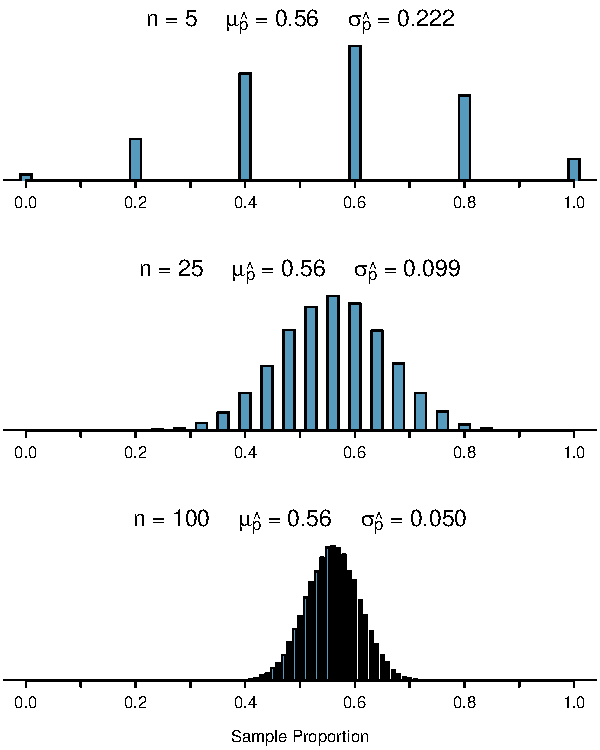
\includegraphics[width=0.67\textwidth]{ch_inference_for_props/figures/sampling_X_prop_56p/sampling_X_prop_56p}
   \caption{Left: simulations of $\hat{p}$ when the sample size
       is $n = 10$ and the population proportion is $p = 0.25$.
       Right: a normal distribution with the same mean (0.25)
       and standard deviation (0.137).}
   \label{sampling_10_prop_25p}
\end{figure}

Notice that the success-failure condition
was not satisfied when $n = 10$ and $p = 0.25$:
\begin{align*}
n p = 10 \times 0.25 = 2.5 &&
    n (1 - p) = 10 \times 0.75 = 7.5
\end{align*}
This single sampling distribution does not show that
the success-failure condition is the perfect guideline,
but we have found that the guideline did correctly
identify that the normal distribution was not appropriate.

We can complete several additional simulations, which are
shown in
Figures~\ref{}
and~\ref{}.
As you review these cases, you'll notice a few things:
\begin{enumerate}
\item When either $np$ or $n(1 - p)$ is small, the
    distribution will more \term{discrete}, which means
    \emph{not continuous}.
\item Additionally, when either value is smaller
    than~10, there is evidence skew in the distribution.
\item The larger both $np$ \emph{and} $n(1 - p)$ are,
    the more normal the distribution will appear.
\item When $np$ and $n(1 - p)$ are both very large,
    the distribution discreteness basically disappears,
    and the distribution looks almost perfectly
    like a normal distribution.
\end{enumerate}

So far we've only focused on the symmetry, discreteness,
and symmetry of the distributions. We haven't considered
how the mean and standard error
of the distributions change!
Take a moment to look back at the graphs,
and pay attention to three things:
\begin{enumerate}
\item The centers of the distribution are always at
    the population proportion, $p$, that was used to
    generate the simulation. Because the sampling
    distribution of $\hat{p}$ is always centered at
    the population parameter $p$, it means the sample
    proportion $\hat{p}$ is \term{unbiased} when
    the data are independent and drawn from such
    a population.
\item For a particular population proportion $p$,
    the variability in the sampling distribution
    decreases as the sample size~$n$ becomes larger.
    This will likely align with your intuition:
    an estimate based on a larger sample size will
    tend to be more accurate.
\item For a particular sample size, the variability
    will be largest when $p = 0.5$. It will be
    easiest to see this for the larger sample sizes.
    This is why the proportion $p$ is used when we
    compute the standard error in the formula:
    $SE = \sqrt{\frac{p (1 - p)}{n}}$.
\end{enumerate}

At no point will the distribution of $\hat{p}$ look
\emph{perfectly} normal.
It is always a matter of degree, and we will use
the standard success-failure condition with minimums
of 10 for $np$ and $n (1 - p)$ as our guideline
within this~book.







%__________________
\section[Inference for other estimators]
    {Inference for other estimators
    \sectionvideohref{youtube-PUMBNtVKr_g&list=PLkIselvEzpM7Pjo94m1e7J5jkIZkbQAl4}~\sectionslideshref{gdoc_os3_slides_4-5}}
\label{aFrameworkForInference}

The sample proportion is not the only point estimate
for which the sampling distribution is nearly normal.
For example, the sampling distribution of sample means
closely resembles the normal distribution when the
sample size is sufficiently large.
In this section, we introduce a number of examples
where the normal approximation is reasonable for
the point estimate.
Chapters~\ref{inferenceForCategoricalData}
and~\ref{inferenceForNumericalData}
revisit each of the point estimates you see in this
section along with some other new statistics.

We make another important assumption about each point
estimate encountered in this section:
the estimate is unbiased, meaning the sampling
distribution of the estimate is centered at the
parameter it estimates.
That is, an unbiased estimate does not naturally
over or underestimate the parameter.
Rather, it tends to provide a ``good'' estimate.
The sample proportion $\hat{p}$ is an example of
an unbiased point estimate, as are each of the
examples we introduce in this section.

Finally, we will discuss the general case where
a~point estimate may follow some distribution
other than the normal distribution. We also provide
guidance about how to handle scenarios where the
statistical techniques you are familiar with are
insufficient for the problem at hand.


\subsection{Confidence intervals for nearly normal
    point estimates}

\index{confidence interval!using normal model|(}

In Section~\ref{confidenceIntervals},
we used the point estimate $\hat{p}$ with
a~standard error $SE_{\hat{p}}$ to create
a 95\% confidence interval for the population
proportion:
\begin{align*}
\hat{p}\ \pm\ 1.96 \times SE_{\hat{p}}
%\label{95PercCIForPHatInGeneralizingSection}
\end{align*}
We constructed this interval by noting that the
sample proportion is within 1.96 standard errors
of the actual proportion about 95\% of the time.
This same logic generalizes to any unbiased point
estimate that closely follows a normal distribution.
We may also generalize the confidence level further
by using a place-holder $z^{\star}$.

\begin{termBox}{\tBoxTitle{General confidence interval
    for the normal sampling distribution case}
    \label{generalConfidenceIntervalTermBox}%
  A confidence interval based on an unbiased and nearly
  normal point estimate is
  \begin{align}
  \text{point estimate}\ \pm\ z^{\star}SE
  \label{95PercGeneralCIInGeneralizingSection}
  \end{align}
  where $z^{\star}$ is selected to correspond to the
  confidence level, and $SE$ represents the standard error
  of the point estimate.
  The value $z^{\star}SE$ is the
  \hiddenterm{margin of error} of the point estimate.}
\end{termBox}

Generally the standard error for a point estimate is
estimated from the data and computed using a formula.
For example, the standard error for the sample
proportion~is
\begin{align*}
SE_{\hat{p}} = \sqrt{\frac{p(1 - p)}{n}}
\end{align*}
In this section, we provide the computed standard error
for each example and exercise without detailing where
the values came from. In future chapters, you will learn
to fill in these and other details for each situation.

\Comment{This next example needs a proper introduction.}

\begin{example}{In Guided Practice~\vref{peOfDiffActiveBetweenGender}, we computed a point estimate for the difference in the average days active per week between male and female students: $\bar{x}_{male}-\bar{x}_{female}=1.1$~days. This point estimate is associated with a nearly normal distribution with standard error $SE = 0.5$~days. What is a reasonable 95\% confidence interval for the difference in average days active per week?}
\label{ciForDiffOfPhysActiveBetweenGenders}
The normal approximation is said to be valid, so we apply Equation~\eqref{95PercGeneralCIInGeneralizingSection}:
\begin{align*}
\text{point estimate}\ \pm\ z^{\star} SE
	\quad\rightarrow\quad 1.1\ \pm\ 1.96\times 0.5
	\quad\rightarrow\quad (0.12, 2.08)
\end{align*}
We are 95\% confident that the male students, on average, were physically active 0.12 to 2.08 days more than female students in YRBSS each week. That is, the actual average difference is plausibly between 0.12 and 2.08 days per week with 95\% confidence.
\end{example}
%library(openintro); library(xtable); data(yrbss); data(yrbss.samp); (x <- by(yrbss.samp$physically_active_7d, yrbss.samp$gender, mean)); diff(x); s <- by(yrbss.samp$physically_active_7d, yrbss.samp$gender, sd); n <- by(yrbss.samp$physically_active_7d, yrbss.samp$gender, length); sqrt(sum(s^2/n))


\begin{example}{Does Example~\ref{ciForDiffOfPhysActiveBetweenGenders} guarantee that if a male and female student are selected at random from YRBSS, the male student would be active 0.12 to 2.08 days more than the female student?}
Our confidence interval says absolutely nothing about individual observations. It {only} makes a statement about a plausible range of values for the \emph{average} difference between all male and female students who participated in YRBSS.
\end{example}

\begin{exercise} \label{findZFor99PercConfLevelInFrameworkForInf}
What $z^{\star}$ would be appropriate for a 99\% confidence level? For help, see Figure~\vref{choosingZForCI}.\footnote{We seek $z^{\star}$ such that 99\% of the area under the normal curve will be between the Z-scores -$z^{\star}$ and $z^{\star}$. Because the remaining 1\% is found in the tails, each tail has area 0.5\%, and we can identify -$z^{\star}$ by looking up 0.0050 in the normal probability table: $z^{\star} = 2.58$. See also Figure~\vref{choosingZForCI}.}
\end{exercise}

\begin{exercise}
The proportion of students who are male in the \data{yrbss\_samp} sample is $\hat{p} = 0.48$. This sample meets certain conditions that ensure $\hat{p}$ will be nearly normal, and the standard error of the estimate is $SE_{\hat{p}} = 0.05$. Create a 90\% confidence interval for the proportion of students in the 2013 YRBSS survey who are male.\footnote{We use $z^{\star}=1.65$ (see Guided Practice~~\vref{find90CIForYrbssAgeExercise}), and apply the general confidence interval formula:
\begin{eqnarray*}
\hat{p}\ \pm\ z^{\star}SE_{\hat{p}}
	\quad\to\quad 0.48\ \pm\ 1.65\times 0.05
	\quad\to\quad (0.3975, 0.5625)
\end{eqnarray*}
Thus, we are 90\% confident that between 40\% and 56\% of the YRBSS students were male.}
\index{confidence interval!using normal model|)}
\end{exercise}


\subsection{Hypothesis testing for nearly normal point estimates}
\index{hypothesis testing!using normal model|(}

Just as the confidence interval method works with many other point estimates, we can generalize our hypothesis testing methods to new point estimates. Here we only consider the p-value approach, introduced in Section~\ref{pValue}, since it is the most commonly used technique and also extends to non-normal cases.

\begin{termBox}{\tBoxTitle[]{Hypothesis testing using the normal model}
\begin{enumerate}
\setlength{\itemsep}{0mm}
\item First write the hypotheses in plain language, then set them up in mathematical notation.
\item Identify an appropriate point estimate of the parameter of interest.
\item Verify conditions to ensure the standard error estimate is reasonable and the point estimate is nearly normal and unbiased.
\item Compute the standard error. Draw a picture depicting the distribution of the estimate under the idea that $H_0$ is true. Shade areas representing the p-value.
\item Using the picture and normal model, compute the \emph{test statistic} (Z-score) and identify the p-value to evaluate the hypotheses. Write a conclusion in plain language.
\end{enumerate}}
\end{termBox}

\begin{exercise} \label{fdaHypSetupForSulph}
A drug called sulphinpyrazone was under consideration for use in reducing the death rate in heart attack patients. To determine whether the drug was effective, a set of 1,475 patients were recruited into an experiment and randomly split into two groups: a control group that received a placebo and a treatment group that received the new drug. What would be an appropriate null hypothesis? And the alternative?\footnote{The skeptic's perspective is that the drug does not work at reducing deaths in heart attack patients ($H_0$), while the alternative is that the drug does work ($H_A$).}
\end{exercise}

We can formalize the hypotheses from Guided Practice~\ref{fdaHypSetupForSulph} by letting $p_{control}$ and $p_{treatment}$ represent the proportion of patients who died in the control and treatment groups, respectively. Then the hypotheses can be written as
\begin{eqnarray*}
&&H_0: p_{control} = p_{treatment} \quad\text{(the drug doesn't work)} \quad \\
&&H_A: p_{control} > p_{treatment} \quad\text{(the drug works)}
\end{eqnarray*}
or equivalently,
\begin{eqnarray*}
&&H_0: p_{control} - p_{treatment} = 0 \quad\text{(the drug doesn't work)} \quad \\
&&H_A: p_{control} - p_{treatment} > 0 \quad\text{(the drug works)}
\end{eqnarray*}
Strong evidence against the null hypothesis and in favor of the alternative would correspond to an observed difference in death rates,
\begin{eqnarray*}
\text{point estimate} = \hat{p}_{control} - \hat{p}_{treatment}
\end{eqnarray*}
being larger than we would expect from chance alone. This difference in sample proportions represents a point estimate that is useful in evaluating the hypotheses. 

\begin{example}{We want to evaluate the hypothesis setup from Guided Practice~\ref{fdaHypSetupForSulph} using data from the actual study.\footnote{Anturane Reinfarction Trial Research Group. 1980. Sulfinpyrazone in the prevention of sudden death after myocardial infarction. New England Journal of Medicine 302(5):250-256.} In the control group, 60 of 742 patients died. In the treatment group, 41 of 733 patients died. The sample difference in death rates can be summarized as
\begin{eqnarray*}
\text{point estimate} = \hat{p}_{control} - \hat{p}_{treatment} = \frac{60}{742} - \frac{41}{733} = 0.025
\end{eqnarray*}
This point estimate is nearly normal and is an unbiased estimate of the actual difference in death rates. The standard error of this sample difference is $SE = 0.013$. Evaluate the hypothesis test at a 5\% significance level: $\alpha=0.05$.}
We would like to identify the p-value to evaluate the hypotheses. If the null hypothesis is true, then the point estimate would have come from a nearly normal distribution, like the one shown in Figure~\ref{sulphStudyFindPValueUsingNormalApprox}. The distribution is centered at zero since $p_{control}-p_{treatment}=0$ under the null hypothesis. Because a large positive difference provides evidence against the null hypothesis and in favor of the alternative, the upper tail has been shaded to represent the p-value. We need not shade the lower tail since this is a one-sided test: an observation in the lower tail does not support the alternative hypothesis.

\begin{figure}[bt]
   \centering
   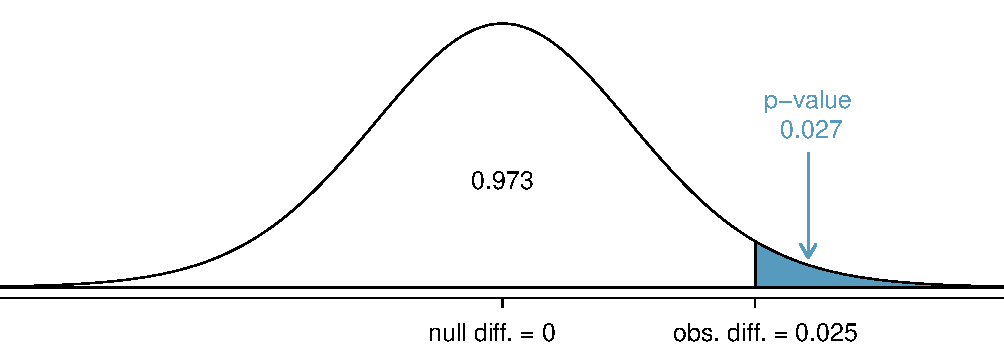
\includegraphics[width=0.88\textwidth]{ch_inference_for_props/figures/sulphStudyFindPValueUsingNormalApprox/sulphStudyFindPValueUsingNormalApprox}
   \caption{The distribution of the sample difference if the null hypothesis is true.}
   \label{sulphStudyFindPValueUsingNormalApprox}
\end{figure}

The p-value can be computed by using the Z-score of the point estimate and the normal probability table.
\begin{eqnarray}
Z = \frac{\text{point estimate} - \text{null value}}{SE_{\text{point estimate}}}
	= \frac{0.025 - 0}{0.013} = 1.92
\label{zScoreOfPointEstimateForSulphinpyrazoneThisIsFirstTestStatReference}
\end{eqnarray}
Examining Z in the normal probability table, we find that the lower unshaded tail is about 0.973. Thus, the upper shaded tail representing the p-value is
\begin{eqnarray*}
\text{p-value} = 1-0.973 = 0.027
\end{eqnarray*}
Because the p-value is less than the significance level ($\alpha=0.05$), we say the null hypothesis is implausible. That is, we reject the null hypothesis in favor of the alternative and conclude that the drug is effective at reducing deaths in heart attack patients.
\end{example}

The Z-score in Equation~(\ref{zScoreOfPointEstimateForSulphinpyrazoneThisIsFirstTestStatReference}) is called a \term{test statistic}. In most hypothesis tests, a test statistic is a particular data summary that is especially useful for computing the p-value and evaluating the hypothesis test. In the case of point estimates that are nearly normal, the test statistic is the Z-score.

\begin{termBox}{\tBoxTitle{Test statistic}
A \emph{test statistic} is a summary statistic that is particularly useful for evaluating a hypothesis test or identifying the p-value. When a point estimate is nearly normal, we use the Z-score of the point estimate as the test statistic. In later chapters we encounter situations where other test statistics are helpful.}
\index{hypothesis testing!using normal model|)}
\end{termBox}


\subsection{Non-normal point estimates}

We may apply the ideas of confidence intervals and hypothesis testing to cases where the point estimate or test statistic is not necessarily normal. There are many reasons why such a situation may arise:
\begin{itemize}
\setlength{\itemsep}{0mm}
\item the sample size is too small for the normal approximation to be valid;
\item the standard error estimate may be poor; or
\item the point estimate tends towards some distribution that is not the normal distribution.
\end{itemize}
For each case where the normal approximation is not valid, our first task is always to understand and characterize the sampling distribution of the point estimate or test statistic. Next, we can apply the general frameworks for confidence intervals and hypothesis testing to these alternative distributions.


\subsection{When to retreat}
\label{whenToRetreat}

Statistical tools rely on conditions. When the conditions are not met, these tools are unreliable and drawing conclusions from them is treacherous. The conditions for these tools typically come in two forms.
\begin{itemize}
\setlength{\itemsep}{0mm}
\item \textbf{The individual observations must be independent.} A random sample from less than 10\% of the population ensures the observations are independent. In experiments, we generally require that subjects are randomized into groups. If independence fails, then advanced techniques must be used, and in some such cases, inference may not be possible.
\item \textbf{Other conditions focus on sample size and skew.} For example, if the sample size is too small, the skew too strong, or extreme outliers are present, then the normal model for the sample mean will fail.
\end{itemize}
Verification of conditions for statistical tools is always necessary. Whenever conditions are not satisfied for a statistical technique, there are three options. The first is to learn new methods that are appropriate for the data. The second route is to consult a data scientist.\footnote{If you work at a university, then there may be campus consulting services to assist you. Alternatively, there are many private consulting firms that are also available for hire.} The third route is to ignore the failure of conditions. This last option effectively invalidates any analysis and may discredit novel and interesting findings.

Finally, we caution that there may be no inference tools helpful when considering data that include unknown biases, such as convenience samples. For this reason, there are books, courses, and researchers devoted to the techniques of sampling and experimental design. See Sections~\ref{overviewOfDataCollectionPrinciples}-\ref{experimentsSection} for basic principles of data collection.


\subsection[Statistical significance versus practical significance]{Statistical significance versus practical significance~\sectionslideshref{gdoc_os3_slides_4-XB}}

When the sample size becomes larger, point estimates become more precise and any real differences in the mean and null value become easier to detect and recognize. Even a very small difference would likely be detected if we took a large enough sample. Sometimes researchers will take such large samples that even the slightest difference is detected. While we still say that difference is \term{statistically significant}, it might not be \term{practically significant}.

Statistically significant differences are sometimes so minor that they are not practically relevant. This is especially important to research: if we conduct a study, we want to focus on finding a meaningful result. We don't want to spend lots of money finding results that hold no practical value.

The role of a data scientist in conducting a study often includes planning the size of the study. The data scientist might first consult experts or scientific literature to learn what would be the smallest meaningful difference from the null value. She also would obtain some reasonable estimate for the standard deviation. With these important pieces of information, she would choose a sufficiently large sample size so that the power for the meaningful difference is perhaps 80\% or 90\%. While larger sample sizes may still be used, she might advise against using them in some cases, especially in sensitive areas of research.












%__________________
\section{One-proportion case studies and sample size calculations}
\label{one_prop_case_studies_and_sample_size_calculations}











%__________________
\section[Difference of two proportions]{Difference of two proportions \sectionvideohref{youtube-_iFAZgpWsx0&feature=youtu.be&t=517&list=PLkIselvEzpM5Gn-sHTw1NF0e8IvMxwHDW}~\sectionslideshref{gdoc_os3_slides_6-2}}
\label{differenceOfTwoProportions}

We would like to make conclusions about the difference in two population proportions: \mbox{$p_1 - p_2$}. We consider three examples. In the first, we compare the approval of the 2010 healthcare law under two different question phrasings. In the second application, we examine the efficacy of mammograms in reducing deaths from breast cancer. In the last example, a quadcopter company weighs whether to switch to a higher quality manufacturer of rotor blades.

In our investigations, we first identify a reasonable point estimate of $p_1 - p_2$ based on the sample. You may have already guessed its form: $\hat{p}_1 - \hat{p}_2$\index{point estimate!difference of proportions}. Next, in each example we verify that the point estimate follows the normal model by checking certain conditions. Finally, we compute the estimate's standard error and apply our inferential framework.


\subsection{Sample distribution of the difference of two proportions}

We must check two conditions before applying the normal model to $\hat{p}_1 - \hat{p}_2$. First, the sampling distribution for each sample proportion must be nearly normal, and secondly, the samples must be independent. Under these two conditions, the sampling distribution of $\hat{p}_1 - \hat{p}_2$ may be well approximated using the normal model.

\begin{termBox}{\tBoxTitle{Conditions for the sampling distribution of $\hat{p}_1 - \hat{p}_2$ to be normal}
The difference $\hat{p}_1 - \hat{p}_2$ tends to follow a normal model when
\begin{itemize}
\setlength{\itemsep}{0mm}
\item each proportion separately follows a normal model, and
\item the two samples are independent of each other.
\end{itemize}
The standard error of the difference in sample proportions is
\index{standard error (SE)!difference in proportions}
\begin{eqnarray}
SE_{\hat{p}_1 - \hat{p}_2}
	= \sqrt{SE_{\hat{p}_1}^2 + SE_{\hat{p}_2}^2}
	= \sqrt{\frac{p_1(1-p_1)}{n_1} + \frac{p_2(1-p_2)}{n_2}}
\label{seForDiffOfProp}
\end{eqnarray}
where $p_1$ and $p_2$ represent the population proportions, and $n_1$ and $n_2$ represent the sample sizes.}
\end{termBox}

For the difference in two means, the standard error formula took the following form:
\begin{eqnarray*}
SE_{\bar{x}_{1} - \bar{x}_{2}} = \sqrt{SE_{\bar{x}_1}^2 + SE_{\bar{x}_2}^2}
\end{eqnarray*}
The standard error for the difference in two proportions takes a similar form. The reasons behind this similarity are rooted in the probability theory of Section~\ref{randomVariablesSection}, which is described for this context in Guided Practice~\vref{derivingSEForDiffOfTwoMeansExercise}.


\subsection{Confidence intervals for $p_1 -p_2$}

In the setting of confidence intervals for a difference of two proportions, the two sample proportions are used to verify the success-failure condition and also compute the standard error, just as was the case with a single proportion.

\begin{example}{The way a question is phrased can influence a person's response. For example, Pew Research Center conducted a survey with the following question:\footnote{\oiRedirect{textbook-health_care_bill_2012}{www.people-press.org/2012/03/26/public-remains-split-on-health-care-bill-opposed-to-mandate}. Sample sizes for each polling group are approximate.}
\begin{quote}
As you may know, by 2014 nearly all Americans will be required to have health insurance. [People who do not buy insurance will pay a penalty] while [People who cannot afford it will receive financial help from the government]. Do you approve or disapprove of this policy?
\end{quote}
\index{data!health care|(}For each randomly sampled respondent, the statements in brackets were randomized: either they were kept in the order given above, or the two statements were reversed. Table~\ref{pewPollResultsForRandomizedStatementOrdering} shows the results of this experiment. Create and interpret a 90\% confidence interval of the difference in approval.}

\begin{table}[t]
\centering
\begin{tabular}{p{50mm}c p{13mm}p{14mm}p{16.5mm}c}
	&\ & Sample size ($n_i$) & Approve law (\%)	& Disapprove law (\%)	& Other \\
\hline
``people who cannot afford it will receive financial help from the government'' is given second \vspace{2.5mm}
	& & 771	& 47	& 49	& 3 \\
``people who do not buy it will pay a penalty'' is given second
	& & 732	& 34	& 63	& 3 \\
\hline
\end{tabular}
\caption{Results for a Pew Research Center poll where the ordering of two statements in a question regarding healthcare were randomized.\vspaceB{-2mm}}
\label{pewPollResultsForRandomizedStatementOrdering}
\end{table}

First the conditions must be verified. Because each group is a simple random sample from less than 10\% of the population, the observations are independent, both within the samples and between the samples. The success-failure condition also holds for each sample. Because all conditions are met, the normal model can be used for the point estimate of the difference in support, where $p_1$ corresponds to the original ordering and $p_2$ to the reversed ordering:
$$\hat{p}_{1} - \hat{p}_{2} = 0.47 - 0.34 = 0.13$$
The standard error may be computed from Equation~\eqref{seForDiffOfProp} using the sample proportions:
$$SE \approx \sqrt{\frac{0.47(1-0.47)}{771} + \frac{0.34(1-0.34)}{732}} = 0.025$$
For a 90\% confidence interval, we use $z^{\star} = 1.65$:
$$\text{point estimate} \ \pm\ z^{\star}SE \quad \to \quad 0.13 \ \pm\ 1.65 \times  0.025 \quad \to \quad (0.09, 0.17)$$
We are 90\% confident that the approval rating for the 2010 healthcare law changes between 9\% and 17\% due to the ordering of the two statements in the survey question. The Pew Research Center reported that this modestly large difference suggests that the opinions of much of the public are still fluid on the health insurance mandate.
\index{data!health care|)}
\end{example}


\subsection{Hypothesis tests for $p_1 -p_2$}

\index{data!mammography|(}
\index{data!breast cancer|(}

A mammogram is an X-ray procedure used to check for breast cancer. Whether mammograms should be used is part of a controversial discussion, and it's the topic of our next example where we examine 2-proportion hypothesis test when $H_0$~is~$p_1 - p_2 = 0$ (or equivalently, $p_1 = p_2$).

A 30-year study was conducted with nearly 90,000 female participants.\footnote{\oiRedirect{textbook-90k_mammogram_study_2014}{Miller AB. 2014. \emph{Twenty five year follow-up for breast cancer incidence and mortality of the Canadian National Breast Screening Study: randomised screening trial}. BMJ 2014;348:g366.}} During a 5-year screening period, each woman was randomized to one of two groups: in the first group, women received regular mammograms to screen for breast cancer, and in the second group, women received regular non-mammogram breast cancer exams. No intervention was made during the following 25 years of the study, and we'll consider death resulting from breast cancer over the full 30-year period. Results from the study are summarized in Table~\ref{mammogramStudySummaryTable}.

If mammograms are much more effective than non-mammogram breast cancer exams, then we would expect to see additional deaths from breast cancer in the control group. On~the other hand, if mammograms are not as effective as regular breast cancer exams, we~would expect to see an increase in breast cancer deaths in the mammogram group.

\begin{table}[h]
\centering
\begin{tabular}{rrcc}
	& \multicolumn{3}{c}{Death from breast cancer?} \\
  \cline{2-4}
 & \ \hspace{3mm}\ & Yes & No \\
  \hline
Mammogram && 500 & 44,425 \\
Control && 505 & 44,405 \\
   \hline
\end{tabular}
\caption{Summary results for breast cancer study.}
\label{mammogramStudySummaryTable}
\end{table}

\begin{exercise}
Is this study an experiment or an observational study?\footnote{This is an experiment. Patients were randomized to receive mammograms or a standard breast cancer exam. We will be able to make causal conclusions based on this study.}
\end{exercise}

\begin{exercise} \label{htFormammogramStudySummaryTable}
Set up hypotheses to test whether there was a difference in breast cancer deaths in the mammogram and control groups.\footnote{$H_0$: the breast cancer death rate for patients screened using mammograms is the same as the breast cancer death rate for patients in the control, $p_{mgm} - p_{ctrl} = 0$. \\ $H_A$: the breast cancer death rate for patients screened using mammograms is different than the breast cancer death rate for patients in the control, $p_{mgm} - p_{ctrl} \neq 0$.}
\end{exercise}

In Example~\ref{condFormammogramStudySummaryTableNormalInference}, we will check the conditions for using the normal model to analyze the results of the study. The details are very similar to that of confidence intervals. However, this time we use a special proportion called the \term{pooled proportion} to check the success-failure condition:
\begin{align*}
\hat{p} &= \frac{\text{\# of patients who died from breast cancer in the entire study}}{\text{\# of patients in the entire study}} \\
	&= \frac{500 + 505}{500 + \text{44,425} + 505 + \text{44,405}} \\
	&= 0.0112
\end{align*}
This proportion is an estimate of the breast cancer death rate across the entire study, and it's our best estimate of the proportions $p_{mgm}$ and $p_{ctrl}$ \emph{if the null hypothesis is true that $p_{mgm} = p_{ctrl}$}. We will also use this pooled proportion when computing the standard error.

\begin{example}{Can we use the normal model to analyze this study?}\label{condFormammogramStudySummaryTableNormalInference}
Because the patients are randomized, they can be treated as independent.

We also must check the success-failure condition for each group. Under the null hypothesis, the proportions $p_{mgm}$ and $p_{ctrl}$ are equal, so we check the success-failure condition with our best estimate of these values under $H_0$, the \hiddenterm{pooled proportion} from the two samples, $\hat{p} = 0.0112$:
\begin{align*}
\hat{p} \times n_{mgm} &= 0.0112 \times \text{44,925} = 503
	& (1 - \hat{p}) \times n_{mgm} &= 0.9888 \times \text{44,925} = \text{44,422} \\
\hat{p} \times n_{ctrl} &= 0.0112 \times \text{44,910} = 503
	& (1 - \hat{p}) \times n_{ctrl} &= 0.9888 \times \text{44,910} = \text{44,407}
\end{align*}
The success-failure condition is satisfied since all values are at least 10, and we can safely apply the normal model.
\end{example}

\begin{termBox}{\tBoxTitle{Use the pooled proportion estimate when $\mathbf{H_0}$ is $\mathbf{p_1 - p_2 = 0}$}
When the null hypothesis is that the proportions are equal, use the pooled proportion ($\hat{p}$) to verify the success-failure condition and estimate the standard error:
\begin{eqnarray*}
\hat{p} = \frac{\text{number of ``successes''}}{\text{number of cases}} = \frac{\hat{p}_1n_1 + \hat{p}_2n_2}{n_1 + n_2}
\end{eqnarray*}
Here $\hat{p}_1n_1$ represents the number of successes in sample 1 since
\begin{eqnarray*}
\hat{p}_1 = \frac{\text{number of successes in sample 1}}{n_1}
\end{eqnarray*}
Similarly, $\hat{p}_2n_2$ represents the number of successes in sample 2.}
\end{termBox}

In Example~\ref{condFormammogramStudySummaryTableNormalInference}, the pooled proportion was used to check the success-failure condition. In the next example, we see the second place where the pooled proportion comes into play: the standard error calculation.

\begin{example}{Compute the point estimate of the difference in breast cancer death rates in the two groups, and use the pooled proportion $\hat{p} = 0.0112$ to calculate the standard error.}
The point estimate of the difference in breast cancer death rates is
\begin{align*}
\hat{p}_{mgm} - \hat{p}_{ctrl}
	&= \frac{500}{500 + 44,425} - \frac{505}{505 + 44,405} \\
	&= 0.01113 - 0.01125 \\
	&= -0.00012
\end{align*}
The breast cancer death rate in the mammogram group was 0.012\% less than in the control group. Next, the standard error is calculated \emph{using the pooled proportion},~$\hat{p}$:
\begin{align*}
SE = \sqrt{\frac{\hat{p}(1-\hat{p})}{n_{mgm}}
		+ \frac{\hat{p}(1-\hat{p})}{n_{ctrl}}}
	= 0.00070
\end{align*}
\end{example}

\begin{example}{Using the point estimate $\hat{p}_{mgm} - \hat{p}_{ctrl} = -0.00012$ and standard error $SE = 0.00070$, calculate a p-value for the hypothesis test and write a conclusion.}
Just like in past tests, we first compute a test statistic and draw a picture:
\begin{align*}
Z = \frac{\text{point estimate} - \text{null value}}{SE}
	= \frac{-0.00012 - 0}{0.00070}
	= -0.17
\end{align*}
\begin{center}
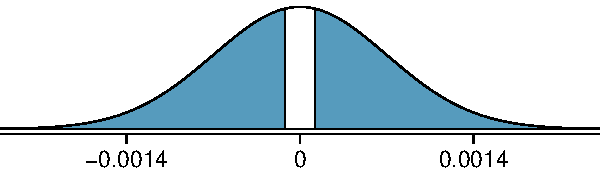
\includegraphics[width=0.6\textwidth]{ch_inference_for_props/figures/mammograms/mammogramPValue}
\end{center}
The lower tail area is 0.4325, which we double to get the p-value:~0.8650. Because this p-value is larger than 0.05, we do not reject the null hypothesis. That is, the difference in breast cancer death rates is reasonably explained by chance, and we do not observe benefits or harm from mammograms relative to a regular breast exam.
\end{example}

Can we conclude that mammograms have no benefits or harm? Here are a few important considerations to keep in mind when reviewing the mammogram study as well as any other medical study:
\begin{itemize}
\setlength{\itemsep}{0mm}
\item If mammograms are helpful or harmful, the data suggest the effect isn't very large. So while we do not accept the null hypothesis, we also don't have sufficient evidence to conclude that mammograms reduce or increase breast cancer deaths.
\item Are mammograms more or less expensive than a non-mammogram breast exam? If~one option is much more expensive than the other and doesn't offer clear benefits, then we should lean towards the less expensive option.
\item The study's authors also found that mammograms led to overdiagnosis of breast cancer, which means some breast cancers were found (or thought to be found) but that these cancers would not cause symptoms during patients' lifetimes. That is, something else would kill the patient before breast cancer symptoms appeared. This means some patients may have been treated for breast cancer unnecessarily, and this treatment is another cost to consider. It is also important to recognize that overdiagnosis can cause unnecessary physical or emotional harm to patients.
\end{itemize}
These considerations highlight the complexity around medical care and treatment recommendations. Experts and medical boards who study medical treatments use considerations like those above to provide their best recommendation based on the current evidence.

\index{data!breast cancer|)}
\index{data!mammography|)}

\CalculatorVideos{confidence intervals and hypothesis tests for the difference of two proportion}


\subsection{More on 2-proportion hypothesis tests (special topic)}

When we conduct a 2-proportion hypothesis test, usually $H_0$ is $p_1 - p_2 = 0$. However, there are rare situations where we want to check for some difference in $p_1$ and $p_2$ that is some value other than 0. For example, maybe we care about checking a null hypothesis where $p_1 - p_2 = 0.1$.\footnote{We can also encounter a similar situation with a difference of two means, though no such example was given in Chapter~\ref{inferenceForNumericalData} since the methods remain exactly the same in the context of sample means. On the other hand, the success-failure condition and the calculation of the standard error vary slightly in different proportion contexts.} In contexts like these, we generally use $\hat{p}_1$ and $\hat{p}_2$ to check the success-failure condition and construct the standard error.

\begin{exercise}\label{carWheelBladeManufacturer}
A quadcopter company is considering a new manufacturer for rotor blades. The new manufacturer would be more expensive but their higher-quality blades are more reliable, resulting in happier customers and fewer warranty claims. However, management must be convinced that the more expensive blades are worth the conversion before they approve the switch. If there is strong evidence of a more than 3\% improvement in the percent of blades that pass inspection, management says they will switch suppliers, otherwise they will maintain the current supplier. Set up appropriate hypotheses for the test.\footnote{$H_0$: The higher-quality blades will pass inspection just 3\% more frequently than the standard-quality blades. $p_{highQ} - p_{standard} = 0.03$. $H_A$: The higher-quality blades will pass inspection $>$3\% more often than the standard-quality blades. $p_{highQ} - p_{standard} > 0.03$.}
\end{exercise}

\setlength{\captionwidth}{85mm}

\begin{figure}
\centering
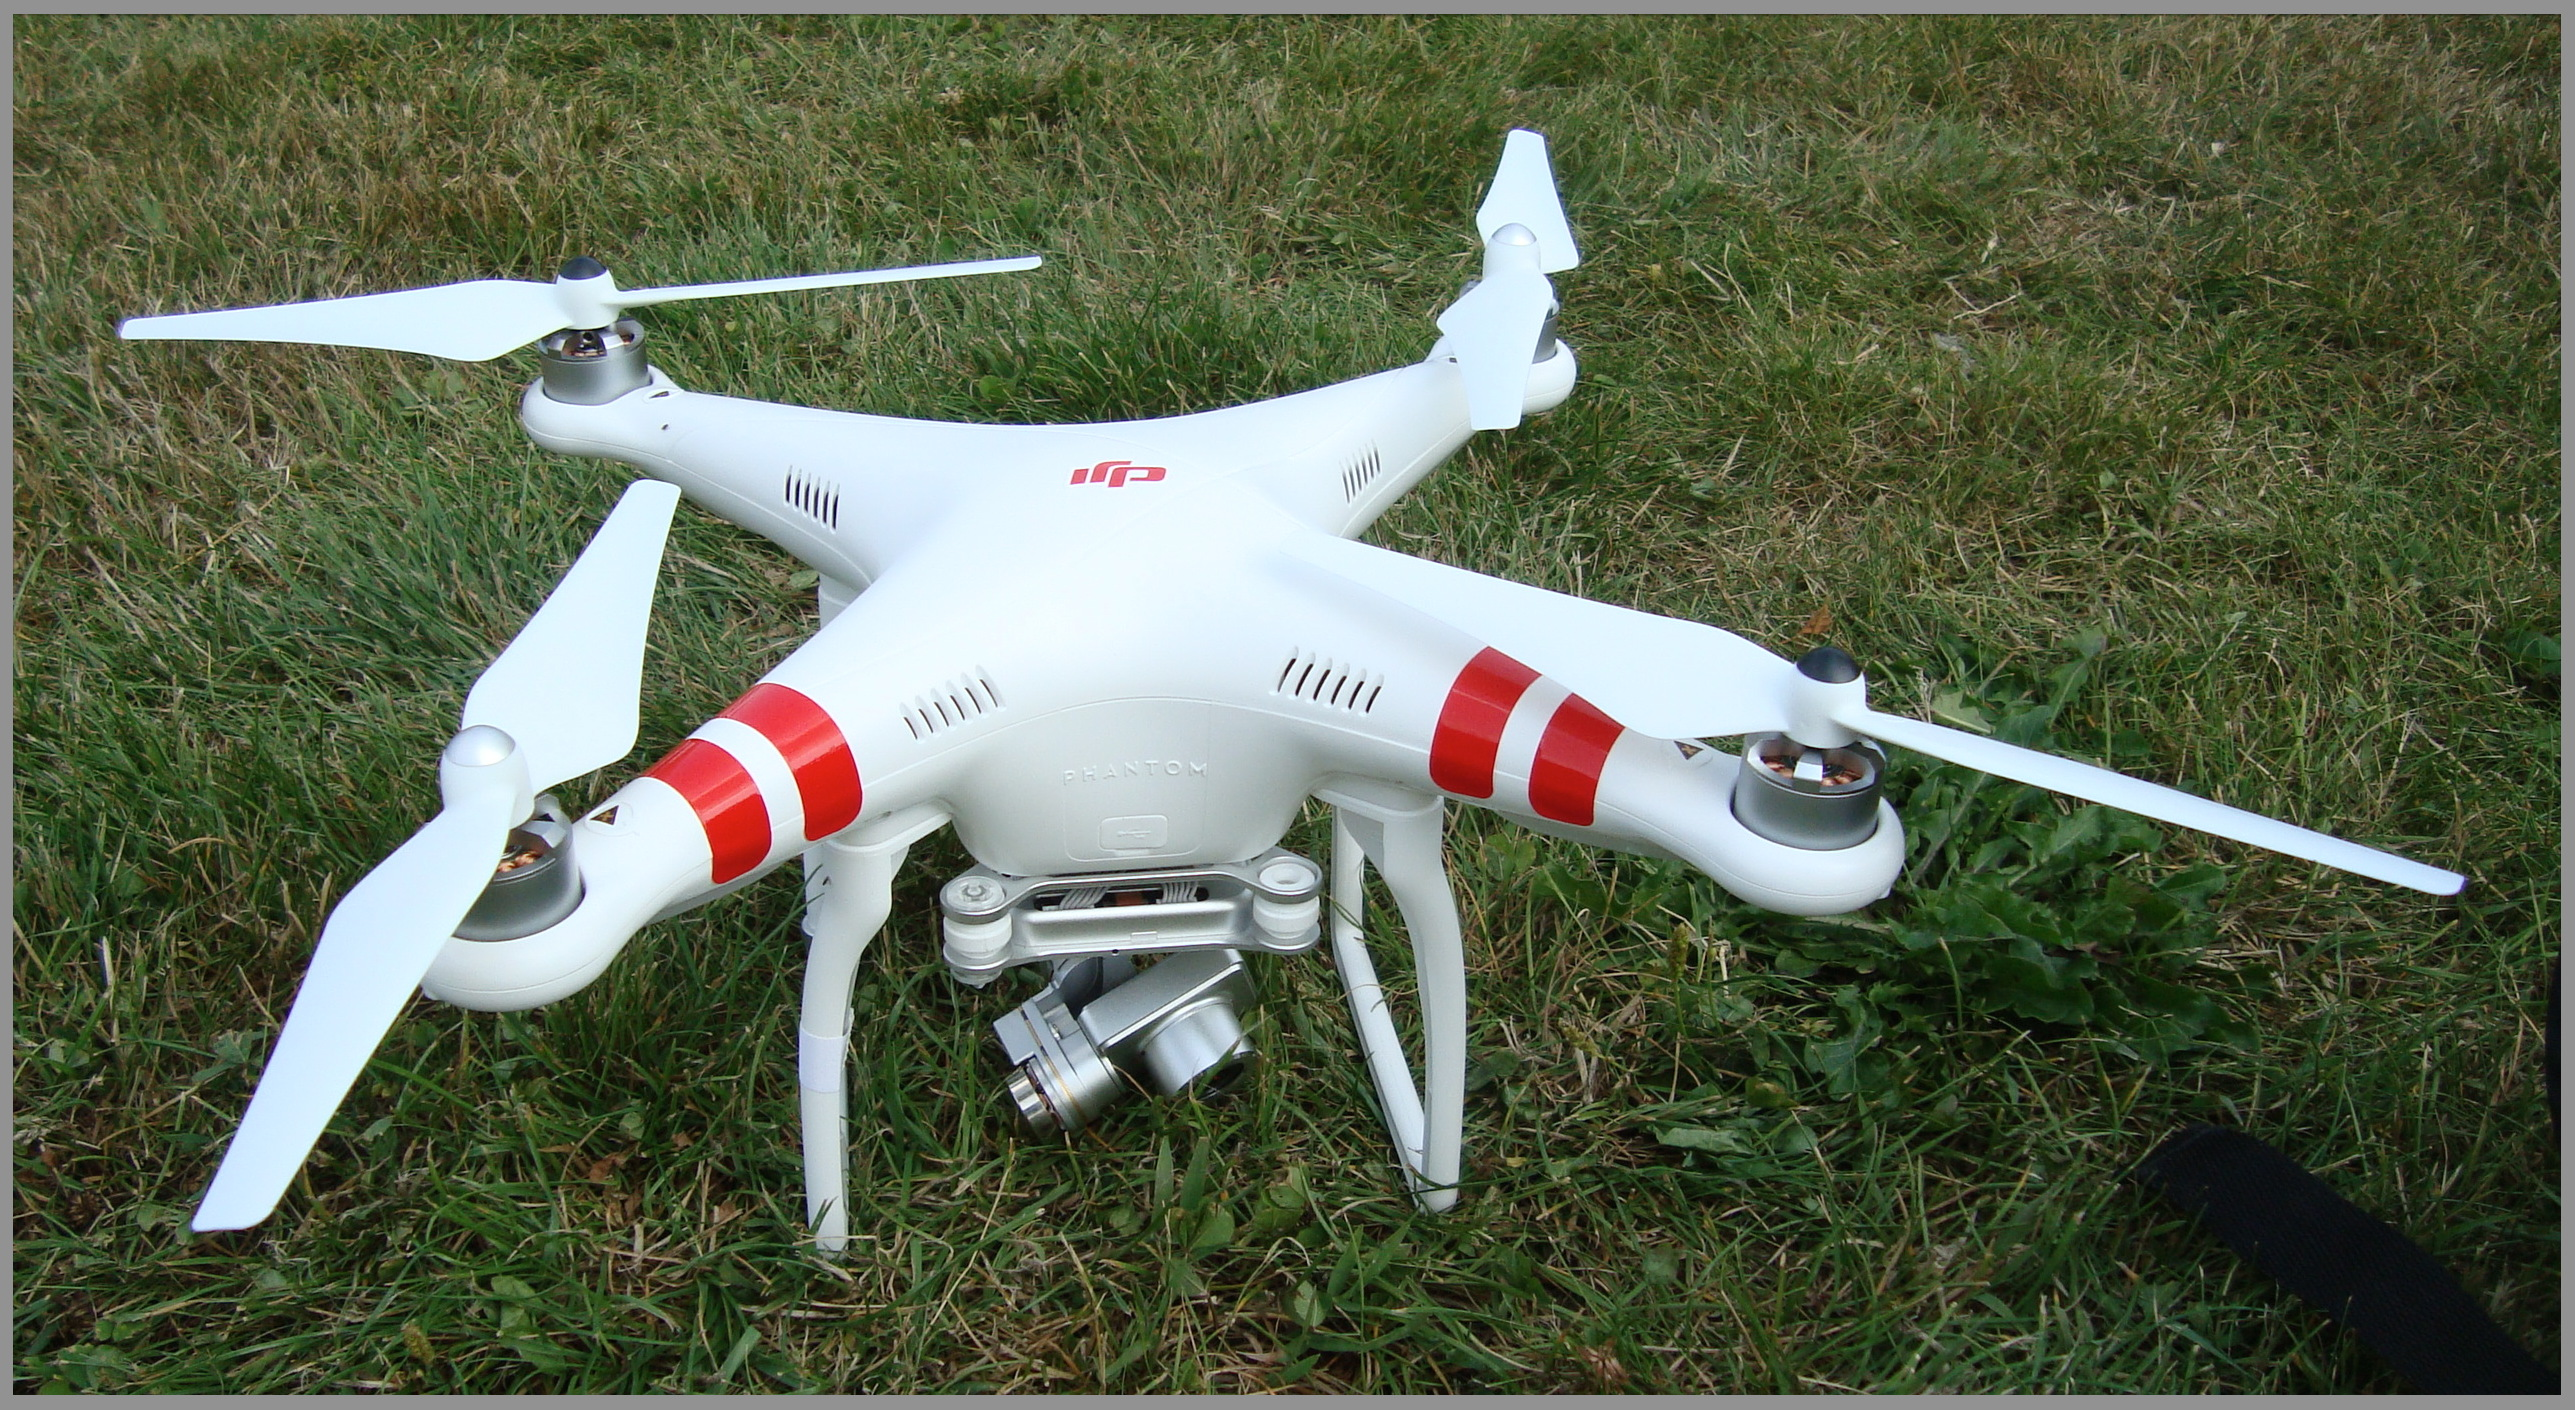
\includegraphics[width=0.6\textwidth]{ch_inference_for_props/figures/quadcopter/quadcopter_david_j}
\caption{A Phantom quadcopter.\vspace{-1mm} \\
   -----------------------------\vspace{-2mm}\\
   {\footnotesize Photo by David J (\oiRedirect{textbook-quadcopter_david_j}{http://flic.kr/p/oiWLNu}). \oiRedirect{textbook-CC_BY_2}{CC-BY 2.0 license.} This photo has been cropped and a border has been added.}}
\label{quadcopter_david_j}
\end{figure}

\setlength{\captionwidth}{\mycaptionwidth}

%\Add{In Guided Practice~\ref{qualityCtrlEngHypothesisEval}, the null difference is 0.03. However, in the vast majority of applications for differences in means or proportions, the null difference is~0. While the details for a difference of means does not change if the null difference is zero or non-zero, that is not the case for a difference in proportions. As we'll see in Section~\ref{}, a hypothesis test for a difference in proportions where the null value is 0 requires additional~care.}

\begin{example}{The quality control engineer from Guided Practice~\ref{carWheelBladeManufacturer} collects a sample of blades, examining 1000 blades from each company and finds that 899 blades pass inspection from the current supplier and 958 pass inspection from the prospective supplier. Using these data, evaluate the hypothesis setup of Guided Practice~\ref{carWheelBladeManufacturer} with a significance level of 5\%.}\label{qualityCtrlEngHypothesisEval}
First, we check the conditions. The sample is not necessarily random, so to proceed we must assume the blades are all independent; for this sample we will suppose this assumption is reasonable, but the engineer would be more knowledgeable as to whether this assumption is appropriate. The success-failure condition also holds for each sample. Thus, the difference in sample proportions, $0.958 - 0.899 = 0.059$, can be said to come from a nearly normal distribution.

The standard error is computed using the two sample proportions since we do not use a pooled proportion for this context:
\begin{align*}
SE = \sqrt{\frac{0.958(1-0.958)}{1000} + \frac{0.899(1-0.899)}{1000}} = 0.0114
\end{align*}
In this hypothesis test, because the null is that $p_1 - p_2 = 0.03$, the sample proportions were used for the standard error calculation rather than a pooled proportion.

Next, we compute the test statistic and use it to find the p-value, which is depicted in Figure~\ref{bladesTwoSampleHTPValueQC}.
$$Z = \frac{\text{point estimate} - \text{null value}}{SE} = \frac{0.059 - 0.03}{0.0114} = 2.54$$
Using the normal model for this test statistic, we identify the right tail area as 0.006. Since this is a one-sided test, this single tail area is also the p-value, and we reject the null hypothesis because 0.006 is less than 0.05. That is, we have statistically significant evidence that the higher-quality blades actually do pass inspection more than 3\% as often as the currently used blades. Based on these results, management will approve the switch to the new supplier.
\end{example}

\begin{figure}
\centering
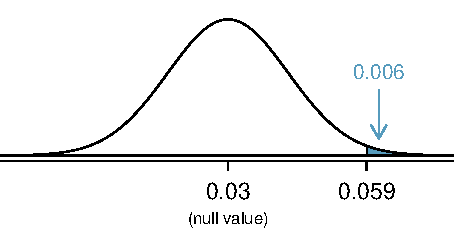
\includegraphics[width=0.5\textwidth]{ch_inference_for_props/figures/bladesTwoSampleHTPValueQC/bladesTwoSampleHTPValueQC}
\caption{Distribution of the test statistic if the null hypothesis was true. The p-value is represented by the shaded area.}
\label{bladesTwoSampleHTPValueQC}
\end{figure}



%%__________________
%\section{Determining a sample size for an experiment}
%\label{SampleSizeFor2Proportions}
%
%So far we've been focused on controlling the Type~1 Error rate for hypothesis tests. However, when planning an experiment, we often are interested in determining if there is an effect.\footnote{Similar planning is also appropriate for a} There are often two competing considerations:
%\begin{itemize}
%\setlength{\itemsep}{0mm}
%\item We want to collect enough data that we can detect important effects.
%\item In many contexts, collecting data is expensive, so we don't want to collect more than what we need to detect effects we care about.
%\end{itemize}
%The first point is relatively simple: the more data we collect, the more precise our estimates will be, and so we'll be able to detect smaller effects. The second point is more subtle, since we need to determine the size of effects that we care about.
%
%%\begin{example}{Alzheimer's disease is a neurological disease. It affects patients mildly at the beginning and eventually leads to dementia. If an Alzheimer's patient lives long enough, the disease will begin affecting bodily functions and ultimately lead to death. It's an extremely serious condition that millions of people, has no cure, and is very expensive to research, partially due to its slow progression. A group of researchers is }
%\begin{example}{}
%
%\end{example}
%
%
%, even large ones, are difficult to detect with small samples, so we should want to collect a larger sample to detect such effects. If we take a very large sample, we might find a statistically significant difference but the magnitude might be so small that it is of no practical value. In this section we describe techniques for selecting an appropriate sample size based on these considerations.





%__________________
\section[Testing for goodness of fit using chi-square (special topic)]{Testing for goodness of fit using chi-square \\(special topic) \sectionvideohref{coursera_video-chisq_gof}~\sectionslideshref{gdoc_os3_slides_6-3}}
\label{oneWayChiSquare}

In this section, we develop a method for assessing a null model when the data are binned.
This technique is commonly used in two circumstances:
\begin{itemize}
\setlength{\itemsep}{0mm}
\item Given a sample of cases that can be classified into several groups, determine if the sample is representative of the general population.
\item Evaluate whether data resemble a particular distribution, such as a normal distribution or a geometric distribution.
\end{itemize}
Each of these scenarios can be addressed using the same statistical test: a chi-square test.

\index{data!racial make-up of jury|(}

In the first case, we consider data from a random sample of 275 jurors in a small county. Jurors identified their racial group, as shown in Table~\ref{juryRepresentationAndCityRepresentationForRace}, and we would like to determine if these jurors are racially representative of the population.  If the jury is representative of the population, then the proportions in the sample should roughly reflect the population of eligible jurors, i.e. registered voters.

\begin{table}[h]
\centering
\begin{tabular}{ll ccc c ll}
\hline
Race	 & \hspace{2mm} & White & Black & Hispanic & Other & \hspace{2mm} & Total \\
\hline
Representation in juries &	& 205 & 26 & 25 & 19 & & 275 \\
Registered voters	 & 		& 0.72 & 0.07 & 0.12 & 0.09 & & 1.00 \\
\hline
\end{tabular}
\caption{Representation by race in a city's juries and population.}
\label{juryRepresentationAndCityRepresentationForRace}
\end{table}

While the proportions in the juries do not precisely represent the population proportions, it is unclear whether these data provide convincing evidence that the sample is not representative. If the jurors really were randomly sampled from the registered voters, we might expect small differences due to chance. However, unusually large differences may provide convincing evidence that the juries were not representative.

A second application, assessing the fit of a distribution, is presented at the end of this section. Daily stock returns from the S\&P500 for the years 1990-2011 are used to assess whether stock activity each day is independent of the stock's behavior on previous days.

In these problems, we would like to examine all bins simultaneously, not simply compare one or two bins at a time, which will require us to develop a new test statistic.


\subsection{Creating a test statistic for one-way tables}

\begin{example}{Of the people in the city, 275 served on a jury. If the individuals are randomly selected to serve on a jury, about how many of the 275 people would we expect to be white? How many would we expect to be black?}
About 72\% of the population is white, so we would expect about 72\% of the jurors to be white: $0.72\times 275 = 198$.

Similarly, we would expect about 7\% of the jurors to be black, which would correspond to about $0.07\times 275 = 19.25$ black jurors.
\end{example}

\begin{exercise}
Twelve percent of the population is Hispanic and 9\% represent other races. How many of the 275 jurors would we expect to be Hispanic or from another race? Answers can be found in Table~\ref{expectedJuryRepresentationIfNoBias}.
\end{exercise}

\begin{table}[h]
\centering
\begin{tabular}{ll ccc c ll}
\hline
Race	 & \hspace{2mm} & White & Black & Hispanic & Other & \hspace{2mm} & Total \\
\hline
Observed data			&	& 205 & 26	& 25 & 19	&	& 275 \\
Expected counts	 &	& 198 & 19.25 & 33 & 24.75 & & 275 \\
\hline
\end{tabular}
\caption{Actual and expected make-up of the jurors.}
\label{expectedJuryRepresentationIfNoBias}
\end{table}

The sample proportion represented from each race among the 275 jurors was not a precise match for any ethnic group. While some sampling variation is expected, we would expect the sample proportions to be fairly similar to the population proportions if there is no bias on juries. We need to test whether the differences are strong enough to provide convincing evidence that the jurors are not a random sample. These ideas can be organized into hypotheses:
\begin{itemize}
\setlength{\itemsep}{0mm}
\item[$H_0$:] The jurors are a random sample, i.e. there is no racial bias in who serves on a jury, and the observed counts reflect natural sampling fluctuation.
\item[$H_A$:] The jurors are not randomly sampled, i.e. there is racial bias in juror selection.
\end{itemize}
To evaluate these hypotheses, we quantify how different the observed counts are from the expected counts. Strong evidence for the alternative hypothesis would come in the form of unusually large deviations in the groups from what would be expected based on sampling variation alone.


\subsection{The chi-square test statistic}
\label{chiSquareTestStatistic}

In previous hypothesis tests, we constructed a test statistic of the following form:
$$ \frac{\text{point estimate} - \text{null value}}{\text{SE of point estimate}} $$
This construction was based on (1) identifying the difference between a point estimate and an expected value if the null hypothesis was true, and (2) standardizing that difference using the standard error of the point estimate. These two ideas will help in the construction of an appropriate test statistic for count data.

Our strategy will be to first compute the difference between the observed counts and the counts we would expect if the null hypothesis was true, then we will standardize the difference:
\begin{align*}
Z_{1} = \frac{\text{observed white count} - \text{null white count}}
				{\text{SE of observed white count}}
\end{align*}
The standard error for the point estimate of the count in binned data is the square root of the count under the null.\footnote{Using some of the rules learned in earlier chapters, we might think that the standard error would be $np(1-p)$, where $n$ is the sample size and $p$ is the proportion in the population. This would be correct if we were looking only at one count. However, we are computing many standardized differences and adding them together. It can be shown -- though not here -- that the square root of the count is a better way to standardize the count differences.} Therefore:
\begin{align*}
Z_1 = \frac{205 - 198}{\sqrt{198}} = 0.50
\end{align*}
The fraction is very similar to previous test statistics: first compute a difference, then standardize it. These computations should also be completed for the black, Hispanic, and other groups:
\begin{align*}
&Black && Hispanic	&&Other \\
& Z_2 = \frac{26-19.25}{\sqrt{19.25}}=1.54\ \ \ \ 
	&& Z_3 = \frac{25-33}{\sqrt{33}}=-1.39\ \ \ \ 
	&& Z_4 = \frac{19-24.75}{\sqrt{24.75}}=-1.16 \\
\end{align*}
We would like to use a single test statistic to determine if these four standardized differences are irregularly far from zero. That is, $Z_1$, $Z_2$, $Z_3$, and $Z_4$ must be combined somehow to help determine if they -- as a group -- tend to be unusually far from zero. A first thought might be to take the absolute value of these four standardized differences and add them~up:
\begin{align*}
|Z_1| + |Z_2| + |Z_3| + |Z_4| = 4.58
\end{align*}
Indeed, this does give one number summarizing how far the actual counts are from what was expected. However, it is more common to add the squared values:
\begin{align*}
Z_1^2 + Z_2^2 + Z_3^2 + Z_4^2 = 5.89
\end{align*}
Squaring each standardized difference before adding them together does two things:
\begin{itemize}
\setlength{\itemsep}{0mm}
\item Any standardized difference that is squared will now be positive.
\item Differences that already look unusual -- e.g. a standardized difference of 2.5 -- will become much larger after being squared.
\end{itemize}
The test statistic $\chi^2$\marginpar[\raggedright\vspace{9mm}

$\chi^2$\vspace{0.5mm}\\\footnotesize chi-square\\test statistic]{\raggedright\vspace{9mm}

$\chi^2$\vspace{0.5mm}\\\footnotesize chi-square\\test statistic},\index{chi-square statistic} which is the sum of the $Z^2$ values, is generally used for these reasons. We can also write an equation for $\chi^2$ using the observed counts and null counts:
\index{data!racial make-up of jury|)}
{\begin{align*}
\chi^2 &=
	\frac
	{\text{\footnotesize$(\text{observed count}_1 - \text{null count}_1)^2$}}
	{\text{\footnotesize$\text{null count}_1$}}
	+ \dots + \frac
	{\text{\footnotesize$(\text{observed count}_4 - \text{null count}_4)^2$}}
	{\text{\footnotesize$\text{null count}_4$}}
\end{align*}
}The final number $\chi^2$ summarizes how strongly the observed counts tend to deviate from the null counts. In Section~\ref{pValueForAChiSquareTest}, we will see that if the null hypothesis is true, then $\chi^2$ follows a new distribution called a \emph{chi-square distribution}. Using this distribution, we will be able to obtain a p-value to evaluate the hypotheses.


\subsection{The chi-square distribution and finding areas}

The \term{chi-square distribution} is sometimes used to characterize data sets and statistics that are always positive and typically right skewed. Recall the normal distribution had two parameters -- mean and standard deviation -- that could be used to describe its exact characteristics. The chi-square distribution has just one parameter called \termsub{degrees of freedom (df)}{degrees of freedom (df)!chi-square}, which influences the shape, center, and spread of the distribution.

\begin{exercise}\label{exerChiSquareDistributionDescriptionWithMoreDOF}
Figure~\ref{chiSquareDistributionWithInceasingDF} shows three chi-square distributions. (a) How does the center of the distribution change when the degrees of freedom is larger? (b) What about the variability (spread)? (c) How does the shape change?\footnote{(a)~The center becomes larger. If took a careful look, we could see that the mean of each distribution is equal to the distribution's degrees of freedom. (b)~The variability increases as the degrees of freedom increases. (c)~The distribution is very strongly skewed for $df=2$, and then the distributions become more symmetric for the larger degrees of freedom $df=4$ and $df=9$. We would see this trend continue if we examined distributions with even more larger degrees of freedom.}
\end{exercise}

\begin{figure}[h]
\centering
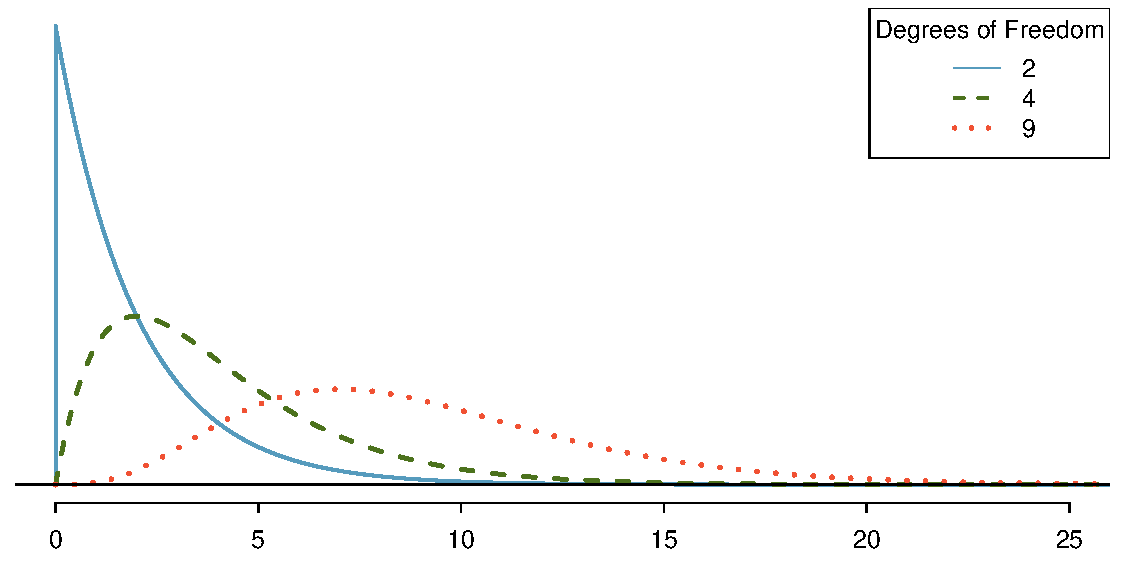
\includegraphics[width=0.9\textwidth]{ch_inference_for_props/figures/chiSquareDistributionWithInceasingDF/chiSquareDistributionWithInceasingDF}
\caption{Three chi-square distributions with varying degrees of freedom.}
\label{chiSquareDistributionWithInceasingDF}
\end{figure}

Figure~\ref{chiSquareDistributionWithInceasingDF} and Guided Practice~\ref{exerChiSquareDistributionDescriptionWithMoreDOF} demonstrate three general properties of chi-square distributions as the degrees of freedom increases: the distribution becomes more symmetric, the center moves to the right, and the variability inflates.

Our principal interest in the chi-square distribution is the calculation of p-values, which (as we have seen before) is related to finding the relevant area in the tail of a distribution. To do so, a new table is needed: the \term{chi-square table}, partially shown in Table~\ref{chiSquareProbabilityTableShort}. A more complete table is presented in Appendix~\vref{chiSquareProbabilityTable}. This table is very similar to the $t$-table: we examine a particular row for distributions with different degrees of freedom, and we identify a range for the area. One important difference from the $t$-table is that the chi-square table only provides upper tail values.

\begin{table}[h]
\centering
\begin{tabular}{r | rrrr | rrrr |}
  \hline
Upper tail & 0.3 & 0.2 & 0.1 & 0.05 & 0.02 & 0.01 & 0.005 & 0.001 \\ 
  \hline
%df \hfill 1 & \footnotesize 1.07 & \footnotesize 1.64 & \footnotesize 2.71 & \footnotesize 3.84 & \footnotesize 5.41 & \footnotesize 6.63 & \footnotesize 7.88 & \footnotesize 10.83 \\ 
df \hfill 2 & \footnotesize 2.41 & \footnotesize \highlightO{3.22} & \footnotesize \highlightO{4.61} & \footnotesize 5.99 & \footnotesize 7.82 & \footnotesize 9.21 & \footnotesize 10.60 & \footnotesize 13.82 \\ 
  \em3 & \em\footnotesize 3.66 & \em\footnotesize 4.64 & \em\footnotesize \highlightT{6.25} & \em\footnotesize 7.81 & \em\footnotesize 9.84 & \em\footnotesize 11.34 & \em\footnotesize 12.84 & \em\footnotesize 16.27 \\ 
  4 & \footnotesize 4.88 & \footnotesize 5.99 & \footnotesize 7.78 & \footnotesize 9.49 & \footnotesize 11.67 & \footnotesize 13.28 & \footnotesize 14.86 & \footnotesize 18.47 \\ 
  5 & \footnotesize 6.06 & \footnotesize 7.29 & \footnotesize 9.24 & \footnotesize 11.07 & \footnotesize 13.39 & \footnotesize 15.09 & \footnotesize 16.75 & \footnotesize 20.52 \\ 
  \hline
  6 & \footnotesize 7.23 & \footnotesize 8.56 & \footnotesize 10.64 & \footnotesize 12.59 & \footnotesize 15.03 & \footnotesize 16.81 & \footnotesize 18.55 & \footnotesize 22.46 \\ 
  7 & \footnotesize 8.38 & \footnotesize 9.80 & \footnotesize 12.02 & \footnotesize 14.07 & \footnotesize 16.62 & \footnotesize 18.48 & \footnotesize 20.28 & \footnotesize 24.32 \\ 
  \hline
\end{tabular}
\caption{A section of the chi-square table. A complete table is in Appendix~\vref{chiSquareProbabilityTable}.}
\label{chiSquareProbabilityTableShort}
\end{table}

\begin{example}{Figure~\ref{chiSquareAreaAbove6Point25WithDF3} shows a chi-square distribution with 3 degrees of freedom and an upper shaded tail starting at 6.25. Use Table~\ref{chiSquareProbabilityTableShort} to estimate the shaded area.}
This distribution has three degrees of freedom, so only the row with 3 degrees of freedom (df) is relevant. This row has been italicized in the table. Next, we see that the value -- 6.25 -- falls in the column with upper tail area 0.1. That is, the shaded upper tail of Figure~\ref{chiSquareAreaAbove6Point25WithDF3} has area 0.1.
\end{example}

\begin{figure}
\centering
\subfigure[]{
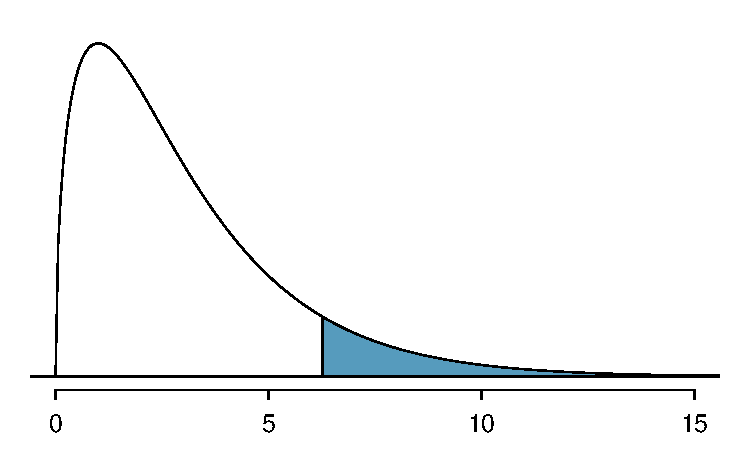
\includegraphics[width=0.475\textwidth]{ch_inference_for_props/figures/arrayOfFigureAreasForChiSquareDistribution/chiSquareAreaAbove6Point25WithDF3/chiSquareAreaAbove6Point25WithDF3}
\label{chiSquareAreaAbove6Point25WithDF3}
}
\subfigure[]{
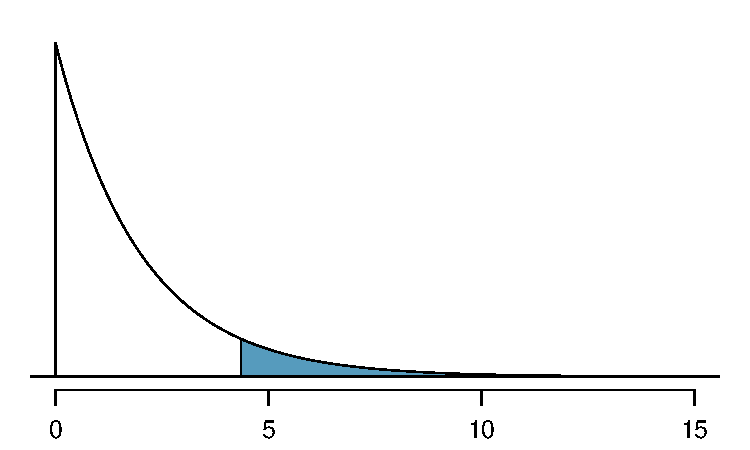
\includegraphics[width=0.475\textwidth]{ch_inference_for_props/figures/arrayOfFigureAreasForChiSquareDistribution/chiSquareAreaAbove4Point3WithDF2/chiSquareAreaAbove4Point3WithDF2}
\label{chiSquareAreaAbove4Point3WithDF2}
}
\subfigure[]{
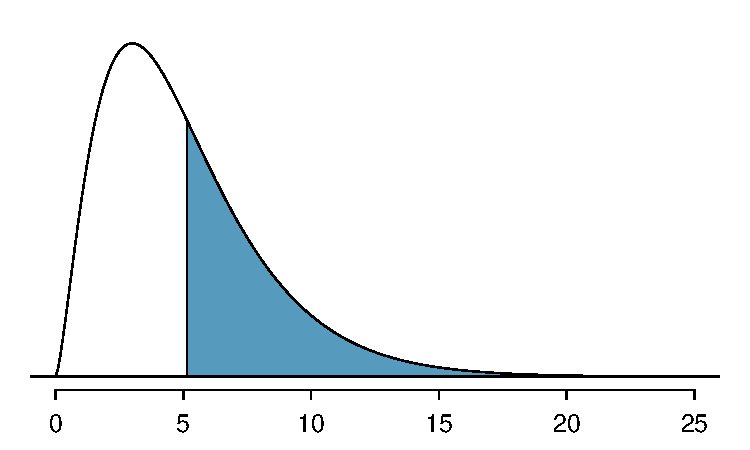
\includegraphics[width=0.475\textwidth]{ch_inference_for_props/figures/arrayOfFigureAreasForChiSquareDistribution/chiSquareAreaAbove5Point1WithDF5/chiSquareAreaAbove5Point1WithDF5}
\label{chiSquareAreaAbove5Point1WithDF5}
}
\subfigure[]{
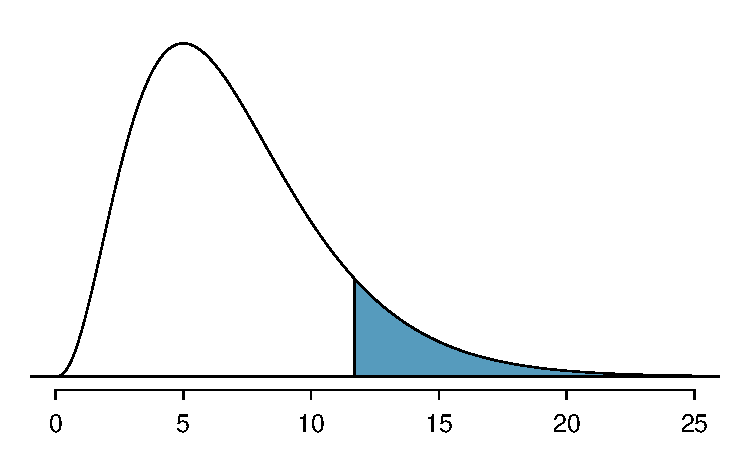
\includegraphics[width=0.475\textwidth]{ch_inference_for_props/figures/arrayOfFigureAreasForChiSquareDistribution/chiSquareAreaAbove11Point7WithDF7/chiSquareAreaAbove11Point7WithDF7}
\label{chiSquareAreaAbove11Point7WithDF7}
}
\subfigure[]{
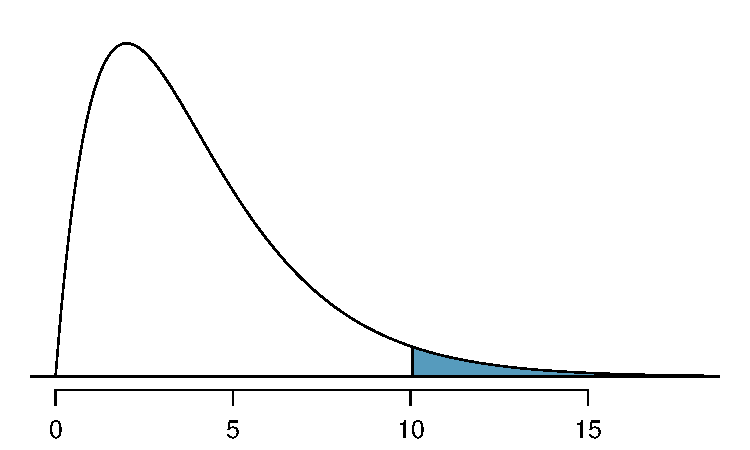
\includegraphics[width=0.475\textwidth]{ch_inference_for_props/figures/arrayOfFigureAreasForChiSquareDistribution/chiSquareAreaAbove10WithDF4/chiSquareAreaAbove10WithDF4}
\label{chiSquareAreaAbove10WithDF4}
}
\subfigure[]{
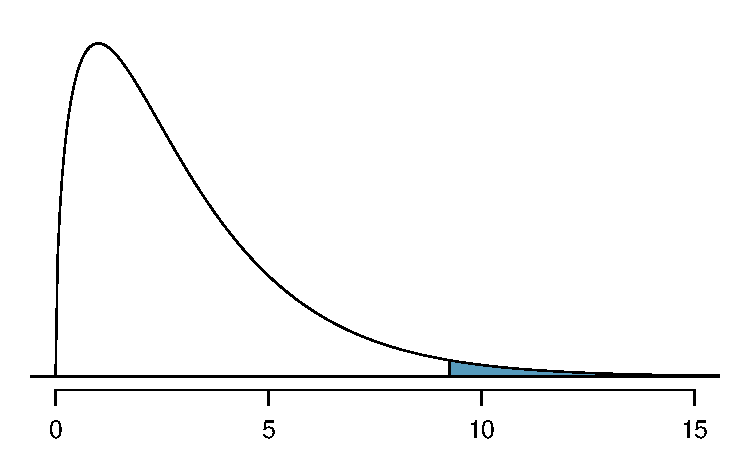
\includegraphics[width=0.475\textwidth]{ch_inference_for_props/figures/arrayOfFigureAreasForChiSquareDistribution/chiSquareAreaAbove9Point21WithDF3/chiSquareAreaAbove9Point21WithDF3}
\label{chiSquareAreaAbove9Point21WithDF3}
}
\caption{
\textbf{\subref{chiSquareAreaAbove6Point25WithDF3}}~Chi-square distribution with 3~degrees of freedom, area above 6.25 shaded.
\textbf{\subref{chiSquareAreaAbove4Point3WithDF2}}~2~degrees of freedom, area above 4.3 shaded.
\textbf{\subref{chiSquareAreaAbove5Point1WithDF5}}~5~degrees of freedom, area above 5.1 shaded.
\textbf{\subref{chiSquareAreaAbove11Point7WithDF7}}~7~degrees of freedom, area above 11.7 shaded.
\textbf{\subref{chiSquareAreaAbove10WithDF4}}~4~degrees of freedom, area above 10 shaded.
\textbf{\subref{chiSquareAreaAbove9Point21WithDF3}}~3~degrees of freedom, area above 9.21 shaded.
}
\label{arrayOfFigureAreasForChiSquareDistribution}
\end{figure}

\begin{example}{We rarely observe the \emph{exact} value in the table. For instance, Figure~\ref{chiSquareAreaAbove4Point3WithDF2} shows the upper tail of a chi-square distribution with 2 degrees of freedom. The bound for this upper tail is at 4.3, which does not fall in Table~\ref{chiSquareProbabilityTableShort}. Find the approximate tail area.}
The cutoff 4.3 falls between the second and third columns in the 2 degrees of freedom row. Because these columns correspond to tail areas of 0.2 and 0.1, we can be certain that the area shaded in Figure~\ref{chiSquareAreaAbove4Point3WithDF2} is between 0.1 and 0.2.
\end{example}

\begin{example}{Figure~\ref{chiSquareAreaAbove5Point1WithDF5} shows an upper tail for a chi-square distribution with 5 degrees of freedom and a cutoff of 5.1. Find the tail area.}
Looking in the row with 5 df, 5.1 falls below the smallest cutoff for this row (6.06). That means we can only say that the area is \emph{greater than 0.3}.
\end{example}

\begin{exercise}
Figure~\ref{chiSquareAreaAbove11Point7WithDF7} shows a cutoff of 11.7 on a chi-square distribution with 7 degrees of freedom. Find the area of the upper tail.\footnote{The value 11.7 falls between 9.80 and 12.02 in the 7 df row. Thus, the area is between 0.1 and 0.2.}
\end{exercise}

\begin{exercise}
Figure~\ref{chiSquareAreaAbove10WithDF4} shows a cutoff of 10 on a chi-square distribution with 4 degrees of freedom. Find the area of the upper tail.\footnote{The area is between 0.02 and 0.05.}
\end{exercise}

\begin{exercise}
Figure~\ref{chiSquareAreaAbove9Point21WithDF3} shows a cutoff of 9.21 with a chi-square distribution with 3 df. Find the area of the upper tail.\footnote{Between 0.02 and 0.05.}
\end{exercise}


\subsection{Finding a p-value for a chi-square distribution}
\label{pValueForAChiSquareTest}

\index{data!racial make-up of jury|(}
In Section~\ref{chiSquareTestStatistic}, we identified a new test statistic ($\chi^2$) within the context of assessing whether there was evidence of racial bias in how jurors were sampled. The null hypothesis represented the claim that jurors were randomly sampled and there was no racial bias. The alternative hypothesis was that there was racial bias in how the jurors were sampled.

We determined that a large $\chi^2$ value would suggest strong evidence favoring the alternative hypothesis: that there was racial bias. However, we could not quantify what the chance was of observing such a large test statistic ($\chi^2=5.89$) if the null hypothesis actually was true. This is where the chi-square distribution becomes useful. If the null hypothesis was true and there was no racial bias, then $\chi^2$ would follow a chi-square distribution, with three degrees of freedom in this case. Under certain conditions, the statistic $\chi^2$ follows a chi-square distribution with $k - 1$ degrees of freedom, where $k$ is the number of bins.

\begin{example}{How many categories were there in the juror example? How many degrees of freedom should be associated with the chi-square distribution used for $\chi^2$?}
In the jurors example, there were $k=4$ categories: white, black, Hispanic, and other. According to the rule above, the test statistic $\chi^2$ should then follow a chi-square distribution with $k-1 = 3$ degrees of freedom if $H_0$ is true.
\end{example}

Just like we checked sample size conditions to use the normal model in earlier sections, we must also check a sample size condition to safely apply the chi-square distribution for $\chi^2$. Each expected count must be at least 5. In the juror example, the expected counts were 198, 19.25, 33, and 24.75, all easily above~5, so we can apply the chi-square model to the test statistic, $\chi^2=5.89$.

\begin{example}{If the null hypothesis is true, the test statistic $\chi^2=5.89$ would be closely associated with a chi-square distribution with three degrees of freedom. Using this distribution and test statistic, identify the p-value.}
The chi-square distribution and p-value are shown in Figure~\ref{jurorHTPValueShown}. Because larger chi-square values correspond to stronger evidence against the null hypothesis, we shade the upper tail to represent the p-value. Using the chi-square table in Appendix~\ref{chiSquareProbabilityTable} or the short table on page~\pageref{chiSquareProbabilityTableShort}, we can determine that the area is between 0.1 and 0.2. That is, the p-value is larger than 0.1 but smaller than 0.2. Generally we do not reject the null hypothesis with such a large p-value. In other words, the data do not provide convincing evidence of racial bias in the juror selection.
\index{data!racial make-up of jury|)}
\end{example}

\begin{figure}[h]
\centering
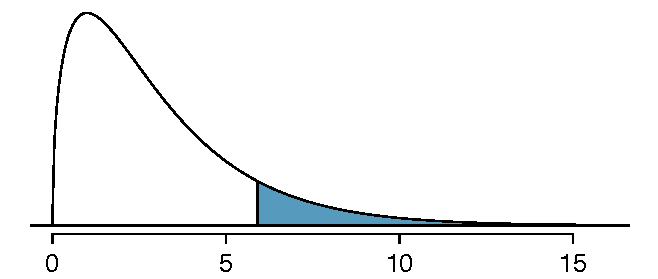
\includegraphics[width=0.55\textwidth]{ch_inference_for_props/figures/jurorHTPValueShown/jurorHTPValueShown}
\caption{The p-value for the juror hypothesis test is shaded in the chi-square distribution with $df=3$.}
\label{jurorHTPValueShown}
\end{figure}

\begin{termBox}{\tBoxTitle{Chi-square test for one-way table}
Suppose we are to evaluate whether there is convincing evidence that a set of observed counts $O_1$, $O_2$, ..., $O_k$ in $k$ categories are unusually different from what might be expected under a null hypothesis. Call the \emph{expected counts} that are based on the null hypothesis $E_1$, $E_2$, ..., $E_k$. If each expected count is at least 5 and the null hypothesis is true, then the test statistic below follows a chi-square distribution with $k-1$ degrees of freedom:
\begin{align*}
\chi^2 = \frac{(O_1 - E_1)^2}{E_1} + \frac{(O_2 - E_2)^2}{E_2} + \cdots + \frac{(O_k - E_k)^2}{E_k}
\end{align*}
The p-value for this test statistic is found by looking at the upper tail of this chi-square distribution. We consider the upper tail because larger values of $\chi^2$ would provide greater evidence against the null hypothesis.}
\end{termBox}

\begin{tipBox}{\tipBoxTitle{Conditions for the chi-square test}
There are two conditions that must be checked before performing a chi-square test:\vspace{-1mm}
\begin{description}
\setlength{\itemsep}{0mm}
\item[Independence.] Each case that contributes a count to the table must be independent of all the other cases in the table.
\item[Sample size / distribution.] Each particular scenario (i.e. cell count) must have at least 5~expected cases.
\vspace{-1mm}
\end{description}
Failing to check conditions may affect the test's error rates.}
\end{tipBox}

When examining a table with just two bins, pick a single bin and use the one-proportion methods introduced in Section~\ref{singleProportion}.


\subsection{Evaluating goodness of fit for a distribution}

Section~\ref{geomDist} would be useful background reading for this example, but it is not a prerequisite.

\index{data!S\&P500 stock data|(}

We can apply our new chi-square testing framework to the second problem in this section: evaluating whether a certain statistical model fits a data set. Daily stock returns from the S\&P500 for 1990-2011 can be used to assess whether stock activity each day is independent of the stock's behavior on previous days. This sounds like a very complex question, and it is, but a chi-square test can be used to study the problem. We will label each day as \resp{Up} or \resp{Down} (\resp{D}) depending on whether the market was up or down that day. For example, consider the following changes in price, their new labels of up and down, and then the number of days that must be observed before each \resp{Up} day:
\begin{center}\footnotesize
\begin{tabular}{lc ccc ccc ccc cc}
Change in price		&\hspace{-1mm}	& \footnotesize2.52 &
	\footnotesize-1.46 & \footnotesize 0.51 &
	\footnotesize-4.07 & \footnotesize3.36 &
	\footnotesize1.10 &
	\footnotesize-5.46 & \footnotesize-1.03 & \footnotesize-2.99 & \footnotesize1.71 \\
Outcome	 & \hspace{-1mm} &
	Up &
	D & Up &
	D & Up &
	Up &
	D & D & D & Up \\
\footnotesize Days to Up & \hspace{-1mm} & 1 & - & 2 & - & 2 & 1 & - & - & - & 4 \\
\end{tabular}
\end{center}
If the days really are independent, then the number of days until a positive trading day should follow a geometric distribution. The geometric distribution describes the probability of waiting for the $k^{th}$ trial to observe the first success. Here each up day (Up) represents a success, and down (D) days represent failures. In the data above, it took only one day until the market was up, so the first wait time was 1 day. It took two more days before we observed our next \resp{Up} trading day, and two more for the third \resp{Up} day. We would like to determine if these counts (1, 2, 2, 1, 4, and so on) follow the geometric distribution. Table~\ref{sAndP500For1990To2011TimeToPosTrade} shows the number of waiting days for a positive trading day during 1990-2011 for the S\&P500.

\begin{table}[h]
\centering
\begin{tabular}{ll ccc ccc c ll}
\hline
Days	 & \hspace{2mm} & 1 & 2 & 3 & 4 & 5 & 6 & 7+ & \hspace{2mm} & Total \\
Observed &		& 1532 & 760 & 338 & 194 & 74 & 33 & 17 & & 2948 \\
\hline
\end{tabular}
\caption{Observed distribution of the waiting time until a positive trading day for the S\&P500, 1990-2011.}
\label{sAndP500For1990To2011TimeToPosTrade}
\end{table}

We consider how many days one must wait until observing an \resp{Up} day on the S\&P500 stock index. If the stock activity was independent from one day to the next and the probability of a positive trading day was constant, then we would expect this waiting time to follow a \emph{geometric distribution}. We can organize this into a hypothesis framework:
\begin{itemize}
\item[$H_0$:] The stock market being up or down on a given day is independent from all other days. We will consider the number of days that pass until an \resp{Up} day is observed. Under this hypothesis, the number of days until an \resp{Up} day should follow a geometric distribution.
\item[$H_A$:] The stock market being up or down on a given day is not independent from all other days. Since we know the number of days until an \resp{Up} day would follow a geometric distribution under the null, we look for deviations from the geometric distribution, which would support the alternative hypothesis.
\end{itemize}
There are important implications in our result for stock traders: if information from past trading days is useful in telling what will happen today, that information may provide an advantage over other traders.

We consider data for the S\&P500 from 1990 to 2011 and summarize the waiting times in Table~\ref{sAndP500For1990To2011TimeToPosTrade2} and Figure~\ref{geomFitEvaluationForSP500For1990To2011}. The S\&P500 was positive on 53.2\% of those days.

\begin{table}
\centering
\begin{tabular}{ll ccc ccc c ll}
\hline
Days	 & \hspace{1mm} & 1 & 2 & 3 & 4 & 5 & 6 & 7+ & \hspace{1mm} & Total \\
\hline
Observed &		& 1532 & 760 & 338 & 194 & 74 & 33 & 17 & & 2948 \\
Geometric Model &		& 1569 & 734 & 343 & 161 & 75 & 35 & 31 & & 2948 \\
\hline
\end{tabular}
\caption{Distribution of the waiting time until a positive trading day. The expected counts based on the geometric model are shown in the last row. To find each expected count, we identify the probability of waiting $D$ days based on the geometric model ($P(D) = (1-0.532)^{D-1}(0.532)$) and multiply by the total number of streaks, 2948. For example, waiting for three days occurs under the geometric model about $0.468^2\times 0.532 = 11.65\%$ of the time, which corresponds to $0.1165\times 2948 = 343$ streaks.}
\label{sAndP500For1990To2011TimeToPosTrade2}
\end{table}

\begin{figure}
\centering
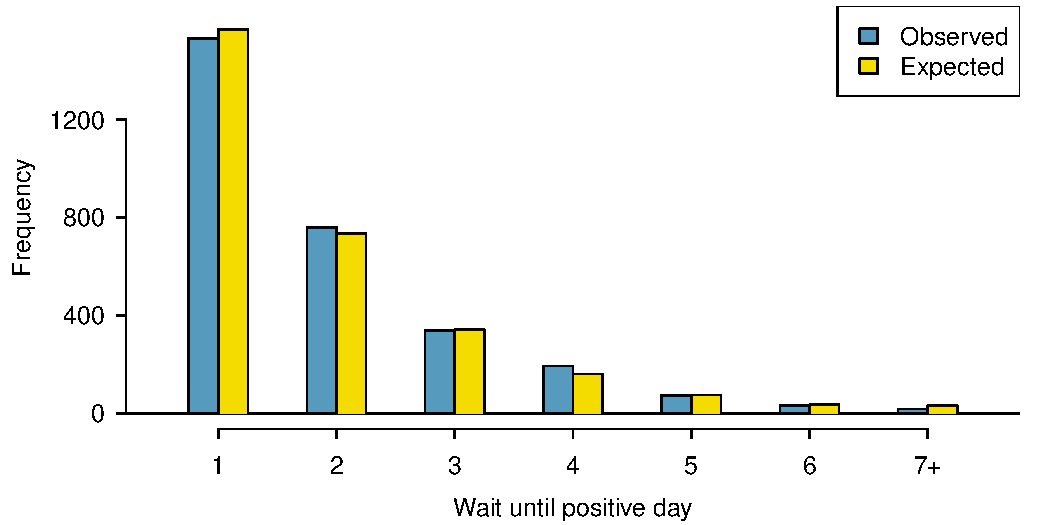
\includegraphics[width=0.98\textwidth]{ch_inference_for_props/figures/geomFitEvaluationForSP500For1990To2011/geomFitEvaluationForSP500For1990To2011}
\caption{Side-by-side bar plot of the observed and expected counts for each waiting time.}
\label{geomFitEvaluationForSP500For1990To2011}
\end{figure}

Because applying the chi-square framework requires expected counts to be at least~5, we have \emph{binned} together all the cases where the waiting time was at least 7 days to ensure each expected count is well above this minimum. The actual data, shown in the \emph{Observed} row in Table~\ref{sAndP500For1990To2011TimeToPosTrade2}, can be compared to the expected counts from the \emph{Geometric Model} row. The method for computing expected counts is discussed in Table~\ref{sAndP500For1990To2011TimeToPosTrade2}. In general, the expected counts are determined by (1) identifying the null proportion associated with each bin, then (2) multiplying each null proportion by the total count to obtain the expected counts. That is, this strategy identifies what proportion of the total count we would expect to be in each bin.

\begin{example}{Do you notice any unusually large deviations in the graph? Can you tell if these deviations are due to chance just by looking?}
It is not obvious whether differences in the observed counts and the expected counts from the geometric distribution are significantly different. That is, it is not clear whether these deviations might be due to chance or whether they are so strong that the data provide convincing evidence against the null hypothesis. However, we can perform a chi-square test using the counts in Table~\ref{sAndP500For1990To2011TimeToPosTrade2}.
\end{example}

\begin{exercise}
Table~\ref{sAndP500For1990To2011TimeToPosTrade2} provides a set of count data for waiting times ($O_1=1532$, $O_2=760$, ...) and expected counts under the geometric distribution ($E_1=1569$, $E_2=734$, ...). Compute the chi-square test statistic, $\chi^2$.\footnote{$\chi^2=\frac{(1532-1569)^2}{1569} + \frac{(760-734)^2}{734} + \cdots + \frac{(17-31)^2}{31} = 15.08$}
\end{exercise}

\begin{exercise}
Because the expected counts are all at least~5, we can safely apply the chi-square distribution to $\chi^2$. However, how many degrees of freedom should we~use?\footnote{There are $k=7$ groups, so we use $df=k-1=6$.}
\end{exercise}

\begin{example}{If the observed counts follow the geometric model, then the chi-square test statistic $\chi^2=15.08$ would closely follow a chi-square distribution with $df=6$. Using this information, compute a p-value.} \label{RejectGeomModelForSP500StockDataFor1990To2011}
Figure~\ref{geomFitPValueForSP500For1990To2011} shows the chi-square distribution, cutoff, and the shaded p-value. If we look up the statistic $\chi^2=15.08$ in Appendix~\ref{chiSquareProbabilityTable}, we find that the p-value is between 0.01 and 0.02. In other words, we have sufficient evidence to reject the notion that the wait times follow a geometric distribution, i.e. trading days are not independent and past days may help predict what the stock market will do today.
\end{example}

\begin{figure}[h]
\centering
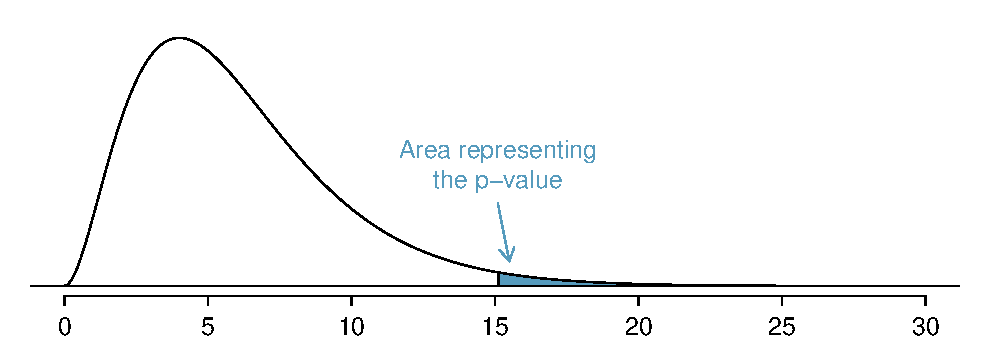
\includegraphics[width=0.9\textwidth]{ch_inference_for_props/figures/geomFitPValueForSP500For1990To2011/geomFitPValueForSP500For1990To2011}
\caption{Chi-square distribution with 6 degrees of freedom. The p-value for the stock analysis is shaded.}
\label{geomFitPValueForSP500For1990To2011}
\end{figure}

\begin{example}{In Example~\ref{RejectGeomModelForSP500StockDataFor1990To2011}, we rejected the null hypothesis that the trading days are independent. Why is this so important?}
Because the data provided strong evidence that the geometric distribution is not appropriate, we reject the claim that trading days are independent. While it is not obvious how to exploit this information, it suggests there are some hidden patterns in the data that could be interesting and possibly useful to a stock trader.
\index{data!S\&P500 stock data|)}
\end{example}

\CalculatorVideos{the chi-square goodness of fit test}



%__________________
\section[Testing for independence in two-way tables (sp. topic)]{Testing for independence in two-way tables\\(special topic) \sectionvideohref{coursera_video-chisq_2way}~\sectionslideshref{gdoc_os3_slides_6-4}}
\label{twoWayTablesAndChiSquare}

\index{data!search algorithm|(}

Google is constantly running experiments to test new search algorithms. For example, Google might test three algorithms using a sample of 10,000 google.com search queries. Table~\ref{googleSearchAlgorithmByAlgorithmOnly} shows an example of 10,000 queries split into three algorithm groups.\footnote{Google regularly runs experiments in this manner to help improve their search engine. It is entirely possible that if you perform a search and so does your friend, that you will have different search results. While the data presented in this section resemble what might be encountered in a real experiment, these data are simulated.} The group sizes were specified before the start of the experiment to be 5000 for the current algorithm and 2500 for each test algorithm.

\begin{table}[h]
\centering
\begin{tabular}{ll ccc ll}
\hline
Search algorithm	 & \hspace{1mm} & current & test 1 & test 2 & \hspace{1mm} & Total \\
Counts &		& 5000 & 2500 & 2500 & & 10000 \\
\hline
\end{tabular}
\caption{Google experiment breakdown of test subjects into three search groups.}
\label{googleSearchAlgorithmByAlgorithmOnly}
\end{table}

\begin{example}{What is the ultimate goal of the Google experiment? What are the null and alternative hypotheses, in regular words?}
The ultimate goal is to see whether there is a difference in the performance of the algorithms. The hypotheses can be described as the following:
\begin{itemize}
\item[$H_0$:] The algorithms each perform equally well.
\item[$H_A$:] The algorithms do not perform equally well.
\end{itemize}
\end{example}

In this experiment, the explanatory variable is the search algorithm. However, an outcome variable is also needed. This outcome variable should somehow reflect whether the search results align with the user's interests. One possible way to quantify this is to determine whether (1)~the user clicked one of the links provided and did not try a new search, or (2)~the user performed a related search. Under scenario~(1), we might think that the user was satisfied with the search results. Under scenario~(2), the search results probably were not relevant, so the user tried a second search.

Table~\ref{googleSearchAlgorithmByAlgorithmAndPerformanceWithTotals} provides the results from the experiment. These data are very similar to the count data in Section~\ref{oneWayChiSquare}. However, now the different combinations of two variables are binned in a \emph{two-way} table. In examining these data, we want to evaluate whether there is strong evidence that at least one algorithm is performing better than the others. To do so, we apply a chi-square test to this two-way table. The ideas of this test are similar to those ideas in the one-way table case. However, degrees of freedom and expected counts are computed a little differently than before.

\begin{table}[h]
\centering
\begin{tabular}{ll ccc ll}
\hline
Search algorithm & \hspace{1mm} & current & test 1 & test 2 & \hspace{1mm} & Total \\
\hline
No new search				   & & 3511    & 1749 & 1818 & 				& 7078 \\
New search				   & & 1489    & 751	& 682    &				& 2922 \\
\hline
Total						   & & 5000    & 2500 & 2500 & 				& 10000 \\
\hline
\end{tabular}
\caption{Results of the Google search algorithm experiment.}
\label{googleSearchAlgorithmByAlgorithmAndPerformanceWithTotals}
\end{table}

\begin{tipBox}{\tipBoxTitle[]{What is so different about one-way tables and two-way tables?}
A one-way table describes counts for each outcome in a single variable. A two-way table describes counts for \emph{combinations} of outcomes for two variables. When we consider a two-way table, we often would like to know, are these variables related in any way? That is, are they dependent (versus independent)?}
\end{tipBox}

The hypothesis test for this Google experiment is really about assessing whether there is statistically significant evidence that the choice of the algorithm affects whether a user performs a second search. In other words, the goal is to check whether the \var{search} variable is independent of the \var{algorithm} variable.


\subsection{Expected counts in two-way tables}

\begin{example}{From the experiment, we estimate the proportion of users who were satisfied with their initial search (no new search) as $7078/10000 = 0.7078$. If there really is no difference among the algorithms and 70.78\% of people are satisfied with the search results, how many of the 5000 people in the ``current algorithm'' group would be expected to not perform a new search?} \label{googleExampleComputingTheExpectedNumberOfCurrentGroupWithNoNewSearch}
About 70.78\% of the 5000 would be satisfied with the initial search:
$$ 0.7078\times 5000 = 3539\text{ users} $$
That is, if there was no difference between the three groups, then we would expect 3539 of the current algorithm users not to perform a new search.
\end{example}

\begin{exercise}\label{googleExampleComputingTheExpectedNumberOfNewAlgGroupWithNoNewSearch}
Using the same rationale described in Example~\ref{googleExampleComputingTheExpectedNumberOfCurrentGroupWithNoNewSearch}, about how many users in each test group would not perform a new search if the algorithms were equally helpful?\footnote{We would expect $0.7078*2500 = 1769.5$. It is okay that this is a fraction.}
\end{exercise}

We can compute the expected number of users who would perform a new search for each group using the same strategy employed in Example~\ref{googleExampleComputingTheExpectedNumberOfCurrentGroupWithNoNewSearch} and Guided Practice~\ref{googleExampleComputingTheExpectedNumberOfNewAlgGroupWithNoNewSearch}. These expected counts were used to construct Table~\ref{googleSearchAlgorithmByAlgorithmAndPerformanceWithExpectedCounts}, which is the same as Table~\ref{googleSearchAlgorithmByAlgorithmAndPerformanceWithTotals}, except now the expected counts have been added in parentheses.

\begin{table}[h]
\centering
\begin{tabular}{l lll lll lll l}
\hline
Search algorithm\hspace{2mm} & \multicolumn{2}{l}{current} &&
					\multicolumn{2}{l}{test 1} &&
					\multicolumn{2}{l}{test 2} & \hspace{0mm} & Total \\
\hline
No new search		   & 3511 &\highlightO{\footnotesize(3539)}    &&
					1749 &\highlightO{\footnotesize(1769.5)}	&&
					1818 &\highlightO{\footnotesize(1769.5)} &	& 7078 \\
New search		   & 1489 &\highlightO{\footnotesize(1461)}    && 
					751 &\highlightO{\footnotesize(730.5)}	&& 
					682 &\highlightO{\footnotesize(730.5)}    &		& 2922 \\
\hline
Total				   & 5000 &&& 	2500 &&& 	2500 &&& 	10000 \\
\hline
\end{tabular}
\caption{The observed counts and the \highlightO{(expected counts)}.}
\label{googleSearchAlgorithmByAlgorithmAndPerformanceWithExpectedCounts}
\end{table}

The examples and exercises above provided some help in computing expected counts. In general, expected counts for a two-way table may be computed using the row totals, column totals, and the table total. For instance, if there was no difference between the groups, then about 70.78\% of each column should be in the first row:
\begin{align*}
0.7078\times (\text{column 1 total}) &= 3539 \\
0.7078\times (\text{column 2 total}) &= 1769.5 \\
0.7078\times (\text{column 3 total}) &= 1769.5
\end{align*}
Looking back to how the fraction 0.7078 was computed -- as the fraction of users who did not perform a new search ($7078/10000$) -- these three expected counts could have been computed as
\begin{align*}
\left(\frac{\text{row 1 total}}{\text{table total}}\right)\text{(column 1 total)} &= 3539 \\
\left(\frac{\text{row 1 total}}{\text{table total}}\right)\text{(column 2 total)} &= 1769.5 \\
\left(\frac{\text{row 1 total}}{\text{table total}}\right)\text{(column 3 total)} &= 1769.5
\end{align*}
This leads us to a general formula for computing expected counts in a two-way table when we would like to test whether there is strong evidence of an association between the column variable and row variable.

\begin{termBox}{\tBoxTitle{Computing expected counts in a two-way table}
To identify the expected count for the $i^{th}$ row and $j^{th}$ column, compute
$$\text{Expected Count}_{\text{row }i,\text{ col }j} = \frac{(\text{row $i$ total}) \times  (\text{column $j$ total})}{\text{table total}}\vspace{2mm}$$}
\end{termBox}


\subsection{The chi-square test for two-way tables}

The chi-square test statistic for a two-way table is found the same way it is found for a one-way table. For each table count, compute
\begin{align*}
&\text{General formula}& &\frac{(\text{observed count } - \text{ expected count})^2}{\text{expected count}} \\
&\text{Row 1, Col 1}& &\frac{(3511 - 3539)^2}{3539} = 0.222 \\
&\text{Row 1, Col 2}& &\frac{(1749 - 1769.5)^2}{1769.5} = 0.237 \\
& \hspace{9mm}\vdots & &\hspace{13mm}\vdots \\
&\text{Row 2, Col 3}& &\frac{(682 - 730.5)^2}{730.5} = 3.220
\end{align*}
Adding the computed value for each cell gives the chi-square test statistic $\chi^2$:
$$\chi^2 = 0.222 + 0.237 + \dots + 3.220 = 6.120$$
Just like before, this test statistic follows a chi-square distribution. However, the degrees of freedom are computed a little differently for a two-way table.\footnote{Recall: in the one-way table, the degrees of freedom was the number of cells minus 1.} For two way tables, the degrees of freedom is equal to
\begin{align*}
df = \text{(number of rows minus 1)}\times \text{(number of columns minus 1)}
\end{align*}
In our example, the degrees of freedom parameter is
\begin{align*}
df = (2-1)\times (3-1) = 2
\end{align*}
If the null hypothesis is true (i.e. the algorithms are equally useful), then the test statistic $\chi^2 = 6.12$ closely follows a chi-square distribution with 2 degrees of freedom. Using this information, we can compute the p-value for the test, which is depicted in Figure~\ref{googleHTForDiffAlgPerformancePValue}.

\begin{termBox}{\tBoxTitle{Computing degrees of freedom for a two-way table}
When applying the chi-square test to a two-way table, we use
$$ df = (R-1)\times (C-1) $$
where $R$ is the number of rows in the table and $C$ is the number of columns.}
\end{termBox}

\begin{tipBox}{\tipBoxTitle{Use two-proportion methods for 2-by-2 contingency tables}
When analyzing 2-by-2 contingency tables, use the two-proportion methods introduced in Section~\ref{differenceOfTwoProportions}.}
\end{tipBox}

\begin{figure}[h]
\centering
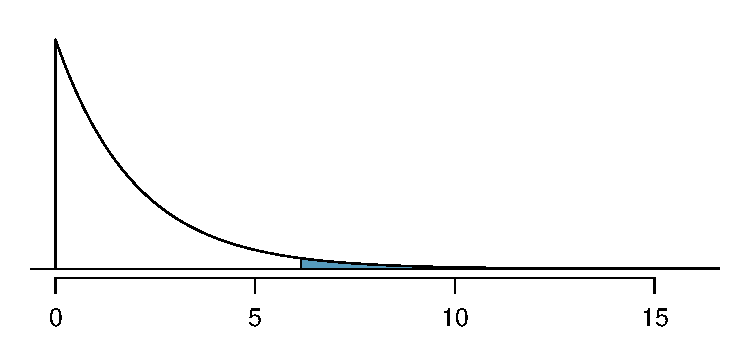
\includegraphics[width=0.7\textwidth]{ch_inference_for_props/figures/googleHTForDiffAlgPerformancePValue/googleHTForDiffAlgPerformancePValue}
\caption{Computing the p-value for the Google hypothesis test.}
\label{googleHTForDiffAlgPerformancePValue}
\end{figure}

\begin{example}{Compute the p-value and draw a conclusion about whether the search algorithms have different performances.}
Looking in Appendix~\ref{chiSquareProbabilityTable} on page~\pageref{chiSquareProbabilityTable}, we examine the row corresponding to 2 degrees of freedom. The test statistic, $\chi^2=6.120$, falls between the fourth and fifth columns, which means the p-value is between 0.02 and 0.05. Because we typically test at a significance level of $\alpha=0.05$ and the p-value is less than 0.05, the null hypothesis is rejected. That is, the data provide convincing evidence that there is some difference in performance among the algorithms.
\index{data!search algorithm|)}
\end{example}

%	Approve	Disapprove
%Obama	56%	41%
%Dem	49%	43%
%Rep	36%	56%
%March 7-11, 2012
%1503 adults

\begin{example}{\index{data!approval ratings|(}Table~\ref{pewResearchPollOnApprovalRatingsForChiSquareSectionExampleAndExercises} summarizes the results of a Pew Research poll.\footnote{See the Pew Research website: \oiRedirect{textbook-obama_and_congress_approval_2012}{www.people-press.org/2012/03/14/romney-leads-gop-contest-trails-in-matchup-with-obama}. The counts in Table~\ref{pewResearchPollOnApprovalRatingsForChiSquareSectionExampleAndExercises} are approximate.} We would like to determine if there are actually differences in the approval ratings of Barack Obama, Democrats in Congress, and Republicans in Congress. What are appropriate hypotheses for such a test?}\label{hypothesisTestSetupForPewResearchPollOnApprovalRatingsForChiSquareSection}
\begin{itemize}
\item[$H_0$:] There is no difference in approval ratings between the three groups.
\item[$H_A$:] There is some difference in approval ratings between the three groups, e.g. perhaps Obama's approval differs from Democrats in Congress.
\end{itemize}
\end{example}

\begin{table}
\centering
\begin{tabular}{ll ccc ll}
& & & \multicolumn{2}{c}{Congress} & \\
\cline{4-5}
 & \hspace{1mm} & Obama & Democrats & Republicans & \hspace{1mm} & Total \\
\hline
Approve				   & & 842    & 736 & 541   & 				& 2119 \\
Disapprove			   & & 616    & 646 & 842   &				& 2104 \\
\hline
Total					   & & 1458    & 1382 & 1383 & 				& 4223 \\
\hline
\end{tabular}
\caption{Pew Research poll results of a March 2012 poll.}
\label{pewResearchPollOnApprovalRatingsForChiSquareSectionExampleAndExercises}
\end{table}

\begin{exercise}
A chi-square test for a two-way table may be used to test the hypotheses in Example~\ref{hypothesisTestSetupForPewResearchPollOnApprovalRatingsForChiSquareSection}. As a first step, compute the expected values for each of the six table cells.\footnote{The expected count for row one / column one is found by multiplying the row one total (2119) and column one total (1458), then dividing by the table total (4223): $\frac{2119\times 1458}{4223} = 731.6$. Similarly for the first column and the second row: $\frac{2104\times 1458}{4223} = 726.4$. Column 2: 693.5 and 688.5. Column 3: 694.0 and 689.0.}
% R <- c(2119, 2104); C <- c(1458, 1382, 1383); R*C[1]/sum(C); R*C[2]/sum(C); R*C[3]/sum(C)
\end{exercise}

\begin{exercise}
Compute the chi-square test statistic.\footnote{For each cell, compute $\frac{(\text{obs} - \text{exp})^2}{exp}$. For instance, the first row and first column: $\frac{(842-731.6)^2}{731.6} = 16.7$. Adding the results of each cell gives the chi-square test statistic: {\scriptsize$\chi^2 = 16.7 + \cdots + 34.0 = 106.4$}.}
%R <- c(2119, 2104); C <- c(1458, 1382, 1383); CC <- c(842, 616, 736, 646, 541, 842); EE <- round(c(R*C[1]/sum(C), R*C[2]/sum(C), R*C[3]/sum(C)), 1); (CC-EE)^2/EE; sum((CC-EE)^2/EE)
\end{exercise}

\begin{exercise}
Because there are 2 rows and 3 columns, the degrees of freedom for the test is $df=(2-1)\times (3-1) = 2$. Use $\chi^2=106.4$, $df=2$, and the chi-square table on page~\pageref{chiSquareProbabilityTable} to evaluate whether to reject the null hypothesis.\footnote{The test statistic is larger than the right-most column of the $df=2$ row of the chi-square table, meaning the p-value is less than 0.001. That is, we reject the null hypothesis because the p-value is less than 0.05, and we conclude that Americans' approval has differences among Democrats in Congress, Republicans in Congress, and the president.}
\index{data!approval ratings|)}
\end{exercise}

\CalculatorVideos{the chi-square test for independence}





